\documentclass[a4paper,12pt]{report}

% Türkçe ve karakter ayarları
\usepackage[utf8]{inputenc}
\usepackage[T1]{fontenc}
\usepackage[turkish]{babel}
\usepackage{lmodern}
\usepackage{geometry}
\usepackage{graphicx}
\usepackage{array}
\usepackage{booktabs}
\usepackage[hidelinks]{hyperref}
\usepackage{longtable}
\usepackage{float}
\usepackage{multirow}
\usepackage {float}

% İstersen Gantt için:
% \usepackage{pgfgantt}

\geometry{margin=2.5cm}

\begin{document}

%-----------------------------
% KAPAK SAYFASI
%-----------------------------
\begin{titlepage}
    \centering
    
    % --- LOGO (HATA VERMEYEN YÖNTEM) ---
    % [width=4cm] parametresini sildik.
    % Yerine \resizebox{4cm}{!} komutuyla dışarıdan boyutlandırdık.
    \resizebox{5cm}{!}{
\includegraphics{gsu-logo.png}}\\[1cm]
    % -----------------------------------
    
    {\Large Galatasaray Üniversitesi}\\[0.5cm]
    {\large Mühendislik ve Teknoloji Fakültesi /  Bilgisayar - Endüstri Mühendisliği INF-493/IND-496 Ortak Projesi}\\[3cm]
    
    {\LARGE \textbf{GSUNET}}\\[2cm]
    
    \textbf{Proje Grubu}\\[0.5cm]
    Mert Samet Kayacıoğlu - 21401923 - Bilgisayar Mühendisliği\\
    Edipcan Erol - 21401938 - Bilgisayar Mühendisliği\\
    Hamza Yakar - 20401896 - Bilgisayar Mühendisliği\\
    Berkay Çadırcı - - Endüstri Mühendisliği\\
    Başar Saraç - - Endüstri Mühendisliği
    
    \vfill
    
    {\large \today}\\
\end{titlepage}

\tableofcontents
\clearpage

%-----------------------------
\chapter{Proje Konusu}

% Projenin genel tanıtımı, problem tanımı, amaç, kapsam vb.

Galatasaray Üniversitesi bünyesinde faaliyet gösteren öğrenci kulüpleri; üniversite kültürünün gelişmesi, öğrencilerin sosyalleşmesi, liderlik becerilerinin güçlenmesi ve organizasyon yetkinliklerinin artırılması açısından önemli bir role sahiptir. Ancak mevcut durumda kulüplerin etkinlik, duyuru ve iletişim süreçleri farklı platformlarda dağınık bir biçimde yürütülmekte olup bu durum hem bilgi kirliliğine hem de koordinasyon eksikliklerine yol açmaktadır.

Etkinlik ve duyuruların çoğu WhatsApp grupları, e-posta zincirleri ve sosyal medya kanalları üzerinden paylaşılmakta; bu nedenle tüm öğrencilere zamanında ulaşmak güçleşmekte ve kulüplerin sürdürülebilir bir dijital hafıza oluşturması mümkün olamamaktadır. Kulüpler arasındaki iletişimin sınırlı olması ise potansiyel işbirliklerinin oluşmasını engellemekte ve öğrenci katılım oranlarını olumsuz etkilemektedir.

Bu ihtiyaçlardan hareketle geliştirilen \textbf{GSUNET (Galatasaray University Networking and Event Tracking System)} projesi, üniversitedeki tüm kulüp, etkinlik ve duyuru süreçlerini tek bir dijital ekosistemde bir araya getirerek bütünleşik ve sürdürülebilir bir yönetim platformu oluşturmayı amaçlamaktadır. GSUNET; öğrencilere, kulüp yöneticilerine, öğretim üyelerine ve sponsor paydaşlarına yönelik çok katmanlı bir yapı sunarak iletişim süreçlerini merkezi bir sistem üzerinden düzenlemeyi hedeflemektedir.

Projenin temel amacı; GSÜ öğrenci topluluklarının etkinlik, duyuru, sponsorluk ve toplantı süreçlerini dijitalleştirerek erişilebilir, verimli ve şeffaf bir yönetim modeli sağlamak, aynı zamanda öğrenci katılımını artırarak üniversitenin sosyal ve kültürel ekosistemini güçlendirmektir.

\section{Projenin Amacı}

GsuNET’in ana hedefi, üniversite kulüplerinin tüm faaliyetlerini tek bir platform üzerinden koordine ederek aşağıdaki faydaları sağlamaktır:

\begin{itemize}
    \item Öğrencilerin etkinliklere hızlı ve kolay erişebilmesi,
    \item Kulüp yönetimlerinin duyuru, etkinlik ve üyelik süreçlerini şeffaf biçimde yönetebilmesi,
    \item Sponsorların kulüplerle doğrudan iletişim kurarak işbirliği olanaklarını değerlendirebilmesi,
    \item Üniversite yönetiminin derslik ve amfi kapasitelerini etkin biçimde organize edebilmesi.
\end{itemize}

Bu platform ile manuel yürütülen süreçler dijital bir yapıya kavuşacak; zaman tasarrufu, kaynak optimizasyonu ve veri temelli karar alma mekanizmaları gelişecektir.

\section{Hedef Kitle ve Kullanıcı Grupları}

\subsection{Öğrenciler}
\begin{itemize}
    \item Etkinliklere kayıt olabilir, kontenjan durumunu görüntüleyebilir.
    \item İlgi alanlarına göre bildirim alabilir.
    \item Katıldığı etkinliklerin geçmişini takip edebilir.
\end{itemize}

\subsection{Kulüp Yönetimleri}
\begin{itemize}
    \item Etkinlik duyurularını ve kayıt süreçlerini yönetebilir.
    \item Sponsorluk talepleri oluşturabilir.
    \item Üyelik ve toplantı takibini gerçekleştirebilir.
\end{itemize}

\subsection{Öğretim Görevlileri / Danışmanlar}
\begin{itemize}
    \item Etkinlik planlarını onaylayabilir veya düzenleme talebi gönderebilir.
    \item Derslik/amfi uygunluğunu gözeterek kapasite planlamasına katkı sağlayabilir.
\end{itemize}

\subsection{Sponsorlar}
\begin{itemize}
    \item Kulüplerin faaliyetlerini inceleyebilir ve sponsorluk teklifinde bulunabilir.
    \item Etkinliklerin hedef kitlesi ve katılım verilerine erişebilir.
\end{itemize}

\section{Proje Kapsamı ve Temel Fonksiyonlar}

\begin{itemize}
    \item \textbf{Etkinlik Yönetim Modülü:} Etkinlik oluşturma, duyuru paylaşımı, kayıt işlemleri ve kapasite takibi.
    \item \textbf{Kulüp Sayfaları:} Her kulüp için tanıtım, geçmiş etkinlikler, yönetim kadrosu ve üyelik bölümü.
    \item \textbf{Toplantı Takip Sistemi:} Aktif toplantıların kaydı, katılım listeleri ve geçmiş toplantı arşivi.
    \item \textbf{Alan Yönetimi:} Derslik ve amfi rezervasyonu; kapasiteye göre otomatik yer önerisi.
    \item \textbf{Sponsorluk Modülü:} Sponsorluk talepleri, teklif eşleştirmeleri ve takip süreçleri.
    \item \textbf{Bildirim ve Takvim Entegrasyonu:} Kişisel takvime etkinlik ekleme ve hatırlatma sistemi.
\end{itemize}


%-----------------------------
\chapter{Proje Planı}

\section{Proje Grubu Yapısı}

% Proje planının ve ana hatlarının oluşturulması (Proje akış şeması, organizasyon şeması vb.)

Proje organizasyonu, Endüstri Mühendisliği ve Bilgisayar Mühendisliği disiplinlerinin ortak çalışmasıyla yürütülmektedir. Yönetim ve teknik süreçlerin koordinasyonu Şekil \ref{fig:org_chart} üzerinde gösterilen organizasyon şemasına göre sağlanmaktadır.

\begin{figure}[htbp]
    \centering
    % width=15cm yerine bu komutu kullanıyoruz.
    % {15cm}{!} -> Genişliği 15cm yap, yüksekliği orantılı (!) ayarla.
    \resizebox{12cm}{!}{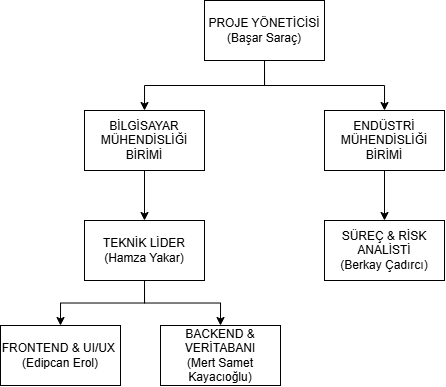
\includegraphics{org-chart.png}}
    \caption{Proje Organizasyon Şeması}
    \label{fig:org_chart}
\end{figure}

Proje ekibi, proje yöneticisi liderliğinde teknik geliştirme ve süreç analizi olmak üzere iki ana kola ayrılmıştır. Bu yapı, disiplinler arası iletişimi güçlendirmekte ve görev dağılımının netleşmesini sağlamaktadır.

\section{Proje Akış Şeması ve Metodoloji}

GsuNET, sürekli geri bildirim ve esneklik sağlayan \textbf{Çevik (Agile)} yöntemle geliştirilmektedir. Şekil \ref{fig:flow_chart}'taki döngüsel akış, her aşamada prototiplerin (MVP) test edilerek nihai ürüne evrilmesini sağlar.

\begin{figure}[htbp]
    \centering
    % { !}{16cm} -> Genişliği orantılı (!) ayarla, yüksekliği 16cm yap.
    \resizebox{!}{18cm}{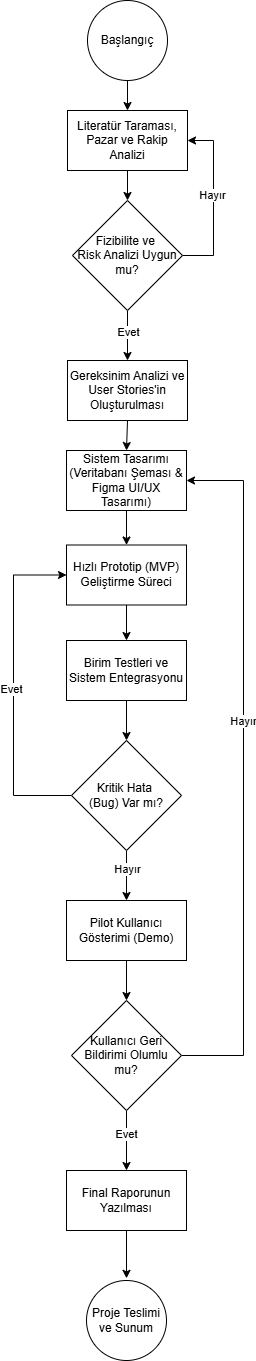
\includegraphics{akis-semasi.png}}
    \caption{GsuNET Proje Genel Akış Şeması}
    \label{fig:flow_chart}
\end{figure}

\chapter{Projedeki Öğrenci Sorumlulukları}

\section{Endüstri Mühendisliği Sorumlulukları}

\begin{itemize}
    \item Genel koordinasyon
    \item İş planlaması
    \item Gantt diyagramı oluşturma
    \item Ekip içi iş bölümü
    \item Sistem analizi
    \item Pazar araştırması
    \item Risk ve fizibilite çalışmaları
    \item Mevcut durum analizi
    \item SWOT değerlendirmesi
\end{itemize}



\section{Bilgisayar Mühendisliği Sorumlulukları}

\begin{itemize}
    \item Kullanıcı arayüzü prototiplerinin hazırlanması
    \item Kullanıcı deneyimi tasarımı
    \item Veritabanı tasarımı
    \item Kullanıcı kayıt sistemi
    \item API entegrasyonu ve sunucu tarafı işlevlerin geliştirilmesi
    \item Web arayüzü ve dinamik sayfaların kodlanması
    \item interaktif kullanıcı deneyimi sağlanması
\end{itemize}


\chapter{Proje Süreci ve Zaman Planı}

GsuNET projesinin zaman planlaması, IND496 ders izlencesinde belirtilen ara rapor ve final raporu teslim tarihleri dikkate alınarak hazırlanmıştır. Gantt şeması, proje sürecini dört ana faz altında toplamaktadır:

\begin{itemize}
    \item Keşif ve İhtiyaç Analizi
    \item Sistem Analizi ve Gereksinim Tanımlama
    \item Sistem Tasarımı ve Demo Geliştirme
    \item Test, Revizyon ve Raporlama
\end{itemize}

Bu fazların her biri hem Endüstri Mühendisliği hem Bilgisayar Mühendisliği öğrencilerinin görev aldığı detaylı aktivitelere ayrılmıştır. Projede kritik görevler önceliklendirilmiş ve ilgili görevler arasında bağımlılıklar tanımlanmıştır.

Aşağıdaki alt bölümlerde, önce proje fazları açıklanmakta, ardından görev listesi ve sorumluluklar, son olarak kritik yol analizi sunulmaktadır.

\section{Proje Fazlarının Ayrıntılı Açıklaması}

GsuNET platform projesi, IND496 dersinin proje gereklilikleri doğrultusunda dört ana faz altında planlanmıştır. Her bir ana faz; analiz, tasarım, geliştirme ve iyileştirme döngüsünü takip ederek hem Endüstri Mühendisliği hem de Bilgisayar Mühendisliği öğrencilerinin sorumluluklarını kapsamaktadır. Fazların kapsamlı açıklamaları;

\subsection{Faz I – Keşif ve İhtiyaç Analizi (Hafta 1–3)}

Bu faz, projenin temelinin atıldığı ve tüm sonraki aşamaların yönünü belirleyen keşif aşamasıdır. Amacı, GsuNET platformunun \textbf{neyi}, \textbf{kim için}, \textbf{hangi problemleri çözmek için} geliştirilmesi gerektiğini netleştirmektir.

Bu fazın çalışmaları:

\begin{itemize}
    \item \textbf{Proje kapsamının tanımlanması:} GsuNET'in amacı, vizyonu, genel çerçevesi, problem alanı ve söz konusu yapının neden gerekli olduğu belirlenir. Platformun üniversite yaşamındaki rolü, çözmeyi hedeflediği operasyonel sıkıntılar ve sağlayacağı değer tanımlanır.

    \item \textbf{Paydaş ve kullanıcı gruplarının belirlenmesi:} Öğrenciler, kulüp yöneticileri, pasif öğrenciler, akademik danışmanlar ve idari birimler belirlenerek paydaş haritası çıkarılır. Her bir paydaşın projeyle etkileşimi ve beklentisi tanımlanır.

    \item \textbf{Mevcut durumun (AS-IS süreçlerinin) analizi:} Halihazırda kulüplerin etkinlik duyurularını, toplantılarını, sponsorluk görüşmelerini ve duyuru akışlarını nasıl yönettiği incelenir. WhatsApp, Instagram, e-posta ve fiziksel afiş gibi dağınık süreçler dokümante edilir. Mevcut durumun sorunları, darboğazları ve belirsizlikleri ortaya konur.

    \item \textbf{Benzer platformların ve literatürün incelenmesi:} Diğer üniversite kulüp yönetim sistemleri araştırılır. Eventbrite, Meetup gibi genel etkinlik platformları analiz edilir. Akademik literatürde kampüs yönetim sistemleri ve öğrenci etkinlik yönetimine dair yaklaşımlar incelenerek proje için referans çerçeve oluşturulur.

    \item \textbf{İlk problem tanımı ve proje hedeflerinin oluşturulması:} Keşif bulguları doğrultusunda probleme dair net bir tanım yapılır. Projenin kısa vadeli (dönem içi) ve uzun vadeli (üniversite ölçeği) hedefleri belirlenir. Bu hedefler, ileride yapılacak sistem analizi çalışmalarına yön sağlar.
\end{itemize}

\textbf{Faz I'in çıktıları:} Projenin kapsam belgesi, paydaş haritası, mevcut süreç akışları (AS-IS), literatür ve benzer sistem inceleme raporu, ilk problem tanımı ve hedef listesi.

Bu faz, proje boyunca alınacak tüm kararlar için \textbf{analitik ve stratejik temel} oluşturduğu için kritik öneme sahiptir.

\subsection{Faz II – Sistem Analizi ve Gereksinim Tanımlama (Hafta 3–6)}

Bu faz, IND496 ara raporunda yer alması zorunlu olan analizlerin tamamlandığı fazdır. Amaç, kullanıcı ihtiyaçlarını sistematik biçimde ortaya koymak ve bunları teknik gereksinimlere dönüştürmektir.

Bu fazın ana çalışmaları:

\begin{itemize}
    \item \textbf{SWOT Analizi:} Platformun güçlü ve zayıf yönleri ile dış çevredeki fırsat ve tehditler belirlenir. Bu analiz proje stratejisinin temelini oluşturur.

    \item \textbf{Pazar Araştırması:} Üniversitelerde kullanılan benzer platformlar incelenir. Var olan etkinlik ve kulüp yönetim araçlarının kapsamı, işlevleri ve eksikleri değerlendirilir.

    \item \textbf{Rekabet Analizi:} Doğrudan rakip (üniversite içi sistemler) ve dolaylı rakip (Instagram, WhatsApp gibi iletişim kanalları) analiz edilir. GsuNET'in farklılaştırıcı yönleri belirlenir.

    \item \textbf{Müşteri Analizi ve Kullanıcı Segmentasyonu:} Kullanıcı grupları detaylı segmentlere ayrılır (kulüp yöneticileri, pasif öğrenciler, akademik danışmanlar, üniversite yönetimi). Her kullanıcının ihtiyaçları, motivasyonları ve platformdaki rolü tanımlanır.

    \item \textbf{Kullanıcı ihtiyaçlarının toplanması:} Anket ve görüşmelerle kullanıcıların gerçek ihtiyaçları belirlenir. Bu veri, QFD çalışmasına girdi olarak kullanılır.

    \item \textbf{Kalite Evi (QFD) çalışması:} Kullanıcı ihtiyaçlarının teknik gereksinimlere dönüştürülmesi sağlanır. Gereksinimler önceliklendirilir.

    \item \textbf{Teknik Fizibilite:} Önerilen teknoloji yığını, altyapı ihtiyaçları ve yazılım mimarisi değerlendirilir.

    \item \textbf{Organizasyonel ve Finansal Fizibilite:} Platformun üniversite içinde sürdürülebilirliği, süreç sahipleri ve maliyet değerlendirmeleri yapılır.

    \item \textbf{Risk Analizi (Risk Matrisi + Senaryo Analizi):} Olasılık–etki matrisine göre riskler belirlenir. Kritik riskler için senaryolar ve aksiyonlar oluşturulur.
\end{itemize}

\textbf{Faz II'nin çıktıları:} SWOT analizi, pazar \& rekabet analizi, müşteri analizi, anket/görüşme bulguları, Kalite Evi (QFD) matrisi, fizibilite raporu, risk matrisi ve senaryo analizi.

Bu faz sonunda projenin analitik çerçevesi tamamen oluşturulmuş olur.

\subsection{Faz III – Sistem Tasarımı ve Demo Geliştirme (Hafta 6–10)}

Bu fazda tasarım ve yazılım geliştirme başlar. Endüstri Mühendisliği öğrencileri gereksinimleri doğrular ve kullanıcı akışlarını kontrol ederken, Bilgisayar Mühendisliği öğrencileri teknik tasarımı ve prototipi geliştirir.

Bu fazın ana çalışmaları:

\begin{itemize}
    \item \textbf{Yüksek seviyeli sistem mimarisinin oluşturulması:} Kullanıcı arayüzü, backend API, veritabanı ve dış entegrasyonlardan (e-posta servisi, bildirim sistemi vb.) oluşan mimari tasarlanır.

    \item \textbf{Veri modelinin (ER diyagramının) oluşturulması:} Kulüpler, etkinlikler, kullanıcılar, sponsorlar, derslikler gibi varlıklar ve aralarındaki ilişkiler tanımlanır.

    \item \textbf{Arayüz prototiplerinin hazırlanması:} Figma veya benzeri araçlarla wireframe ve mockup'lar oluşturulur. Tasarımda kullanıcı yolculuğu (user journey) dikkate alınır.

    \item \textbf{Temel fonksiyonları içeren demo geliştirilmesi:} Etkinlik oluşturma, listeleme, kullanıcı kaydı, rol tanımlama gibi temel özelliklerin çalışır bir versiyonu kodlanır.
\end{itemize}

\textbf{Faz III'ün çıktıları:} Sistem mimari diyagramı, veri modeli (ER diyagramı), arayüz prototipleri, demo prototip yazılımı.

Bu faz sonunda GsuNET platformunun teknik temelleri ve ilk MVP (Minimum Viable Product) tamamlanmış olur.

\subsection{Faz IV – Test, Revizyon ve Raporlama (Hafta 10–12)}

Bu faz, geliştirilen demo sistemin test edildiği, kullanıcı geri bildirimlerine göre iyileştirmelerin yapıldığı ve final raporunun tamamlandığı aşamadır.

Bu fazın ana çalışmaları:

\begin{itemize}
    \item \textbf{Pilot kullanıcı testleri ve geri bildirim toplanması:} Demo prototip, öğrenci, kulüp yöneticisi ve danışman gibi farklı kullanıcı gruplarıyla test edilir. Kullanılabilirlik sorunları, hata raporları ve öneriler kaydedilir.

    \item \textbf{İyileştirme aksiyonlarının uygulanması:} Test sürecinde tespit edilen kritik hatalar giderilir, kullanıcı arayüzü iyileştirmeleri yapılır. Geri bildirimler doğrultusunda fonksiyonel eklemeler veya revizyonlar gerçekleştirilir.

    \item \textbf{Ara rapor, final rapor ve sunum materyallerinin tamamlanması:} Tüm analiz, tasarım, geliştirme ve test süreçleri dokümante edilir. Final raporu ve sunum hazırlanarak teslim edilir.
\end{itemize}

\textbf{Faz IV'ün çıktıları:} Pilot test raporu, revize edilmiş demo yazılımı, ara rapor, final rapor, sunum materyalleri.

Bu faz sonunda proje tamamlanmış ve teslime hazır hale gelmiş olur.

Bu fazlar, ders takviminde belirtilen \textbf{ara rapor (22 Kasım)} ve \textbf{final rapor (19 Aralık)} teslim tarihlerini karşılayacak biçimde haftalara dağıtılmıştır.

\section{Gantt Şeması Görev Listesi}

Tarihler örnek olacak şekilde haftalık ölçekle verilmiştir. Tablo \ref{tab:gantt_tasks}'te proje görevleri, fazları, tahmini süreleri ve sorumlular detaylandırılmıştır.

\begin{longtable}{|p{0.5cm}|p{5cm}|p{1cm}|p{2.5cm}|p{2cm}|p{3cm}|}
\hline
\textbf{No} & \textbf{Görev} & \textbf{Faz} & \textbf{Tarih Aralığı} & \textbf{Sorumlu} & \textbf{Açıklama} \\
\hline
\endfirsthead
\hline
\textbf{No} & \textbf{Görev} & \textbf{Faz} & \textbf{Tarih Aralığı} & \textbf{Sorumlu} & \textbf{Açıklama} \\
\hline
\endhead
\hline
\endfoot

1 & Proje kapsamının netleştirilmesi, problem tanımı & I & Hafta 1 & Tüm ekip & GsuNET'in amacı, hedefleri, kullanıcı grupları ve ana modülleri tanımlanır. \\
\hline

2 & Paydaş ve kullanıcı gruplarının belirlenmesi & I & Hafta 1–2 & Endüstri & Öğrenciler, kulüp yönetimleri, danışmanlar ve idari birimler için paydaş haritası çıkarılır. \\
\hline

3 & Mevcut durumun dokümantasyonu & I & Hafta 2 & Endüstri & GSÜ'de kulüp ve etkinlik süreçlerinin şu anki işleyişi modellenir. \\
\hline

4 & Literatür ve benzer platform taraması & I & Hafta 2–3 & Endüstri & Diğer üniversite sistemleri ve genel etkinlik platformları incelenir. \\
\hline

5 & SWOT analizinin hazırlanması & II & Hafta 3 & Endüstri & GsuNET'in güçlü/zayıf yönleri ile fırsat ve tehditleri belirlenir. \\
\hline

6 & Pazar ve rekabet analizinin yapılması & II & Hafta 3–4 & Endüstri & Rakip sistemler ve alternatif çözümler değerlendirilir. \\
\hline

7 & Müşteri analizi ve kullanıcı segmentasyonu & II & Hafta 4 & Endüstri & Kulüp yöneticisi, pasif öğrenci, danışman, yönetim gibi segmentler tanımlanır. \\
\hline

8 & Kullanıcı ihtiyaçlarının toplanması (anket/görüşme) & II & Hafta 4–5 & Endüstri & Kısa anketler ve/veya görüşmelerle beklentiler toplanır. \\
\hline

9 & Kalite Evi (QFD) çalışmasının yapılması & II & Hafta 5 & Endüstri & Kullanıcı ihtiyaçları teknik tasarım gereksinimlerine dönüştürülür. \\
\hline

10 & Teknik fizibilite analizi & II & Hafta 5 & Endüstri & Önerilen teknoloji yığını, entegrasyon imkânları değerlendirilir. \\
\hline

11 & Organizasyonel ve finansal fizibilite analizi & II & Hafta 5–6 & Endüstri & Kurumsal sahiplenme, insan kaynağı ve maliyetler analiz edilir. \\
\hline

12 & Risk matrisi ve senaryo analizlerinin oluşturulması & II & Hafta 6 & Endüstri & Olasılık–etki değerlendirmesi ve senaryo bazlı tartışmalar yapılır. \\
\hline

13 & Yüksek seviyeli sistem mimarisi taslağının hazırlanması & III & Hafta 5–6 & Bilgisayar & Kullanıcı rolleri, modüller ve ana veri akışı şemalandırılır. \\
\hline

14 & Veri modeli ve veritabanı şeması & III & Hafta 6–7 & Bilgisayar & Kulüp, etkinlik, kullanıcı, sponsorluk vb. için tablo yapıları belirlenir. \\
\hline

15 & Kullanıcı arayüz prototiplerinin (wireframe) oluşturulması & III & Hafta 7–8 & Bilgisayar & Giriş sayfası, kulüp profili, takvim ekranı gibi temel ekranlar tasarlanır. \\
\hline

16 & Ara raporun ilk taslağının yazılması (1–7. maddeler) & II–III & Hafta 6–7 & Tüm ekip & Sistem analizi ve Gantt içeren ara rapor taslağı hazırlanır. \\
\hline

17 & Ara raporun son hâle getirilmesi ve teslimi & III & Hafta 8 & Tüm ekip & Düzeltmeler yapılarak ara rapor koordinatörlere iletilir. \\
\hline

18 & Temel demo fonksiyonlarının geliştirilmesi & III & Hafta 8–10 & Bilgisayar & Platformun çalışır bir prototipi oluşturulur (login, kulüp sayfası, etkinlik oluşturma). \\
\hline

19 & Pilot kullanıcı testlerinin yapılması & IV & Hafta 10–11 & Tüm ekip & Seçilen kulüpler ve öğrencilerle kısa kullanıcı testleri gerçekleştirilir. \\
\hline

20 & Test sonrası iyileştirme ve son revizyonlar & IV & Hafta 11–12 & Tüm ekip & Geri bildirimlere göre tasarım ve fonksiyonlar iyileştirilir. \\
\hline

21 & Final raporu ve sunumunun hazırlanması & IV & Hafta 11–12 & Tüm ekip & IEEE formatına uygun rapor ve demo sunumu tamamlanır. \\
\hline

\caption{GsuNET Proje Görev Listesi}
\label{tab:gantt_tasks}
\end{longtable}

\begin{figure}[htbp]
    \centering
    % Ünlem işareti (!) genişliği otomatik oranla demektir.
    \resizebox{!}{6cm}{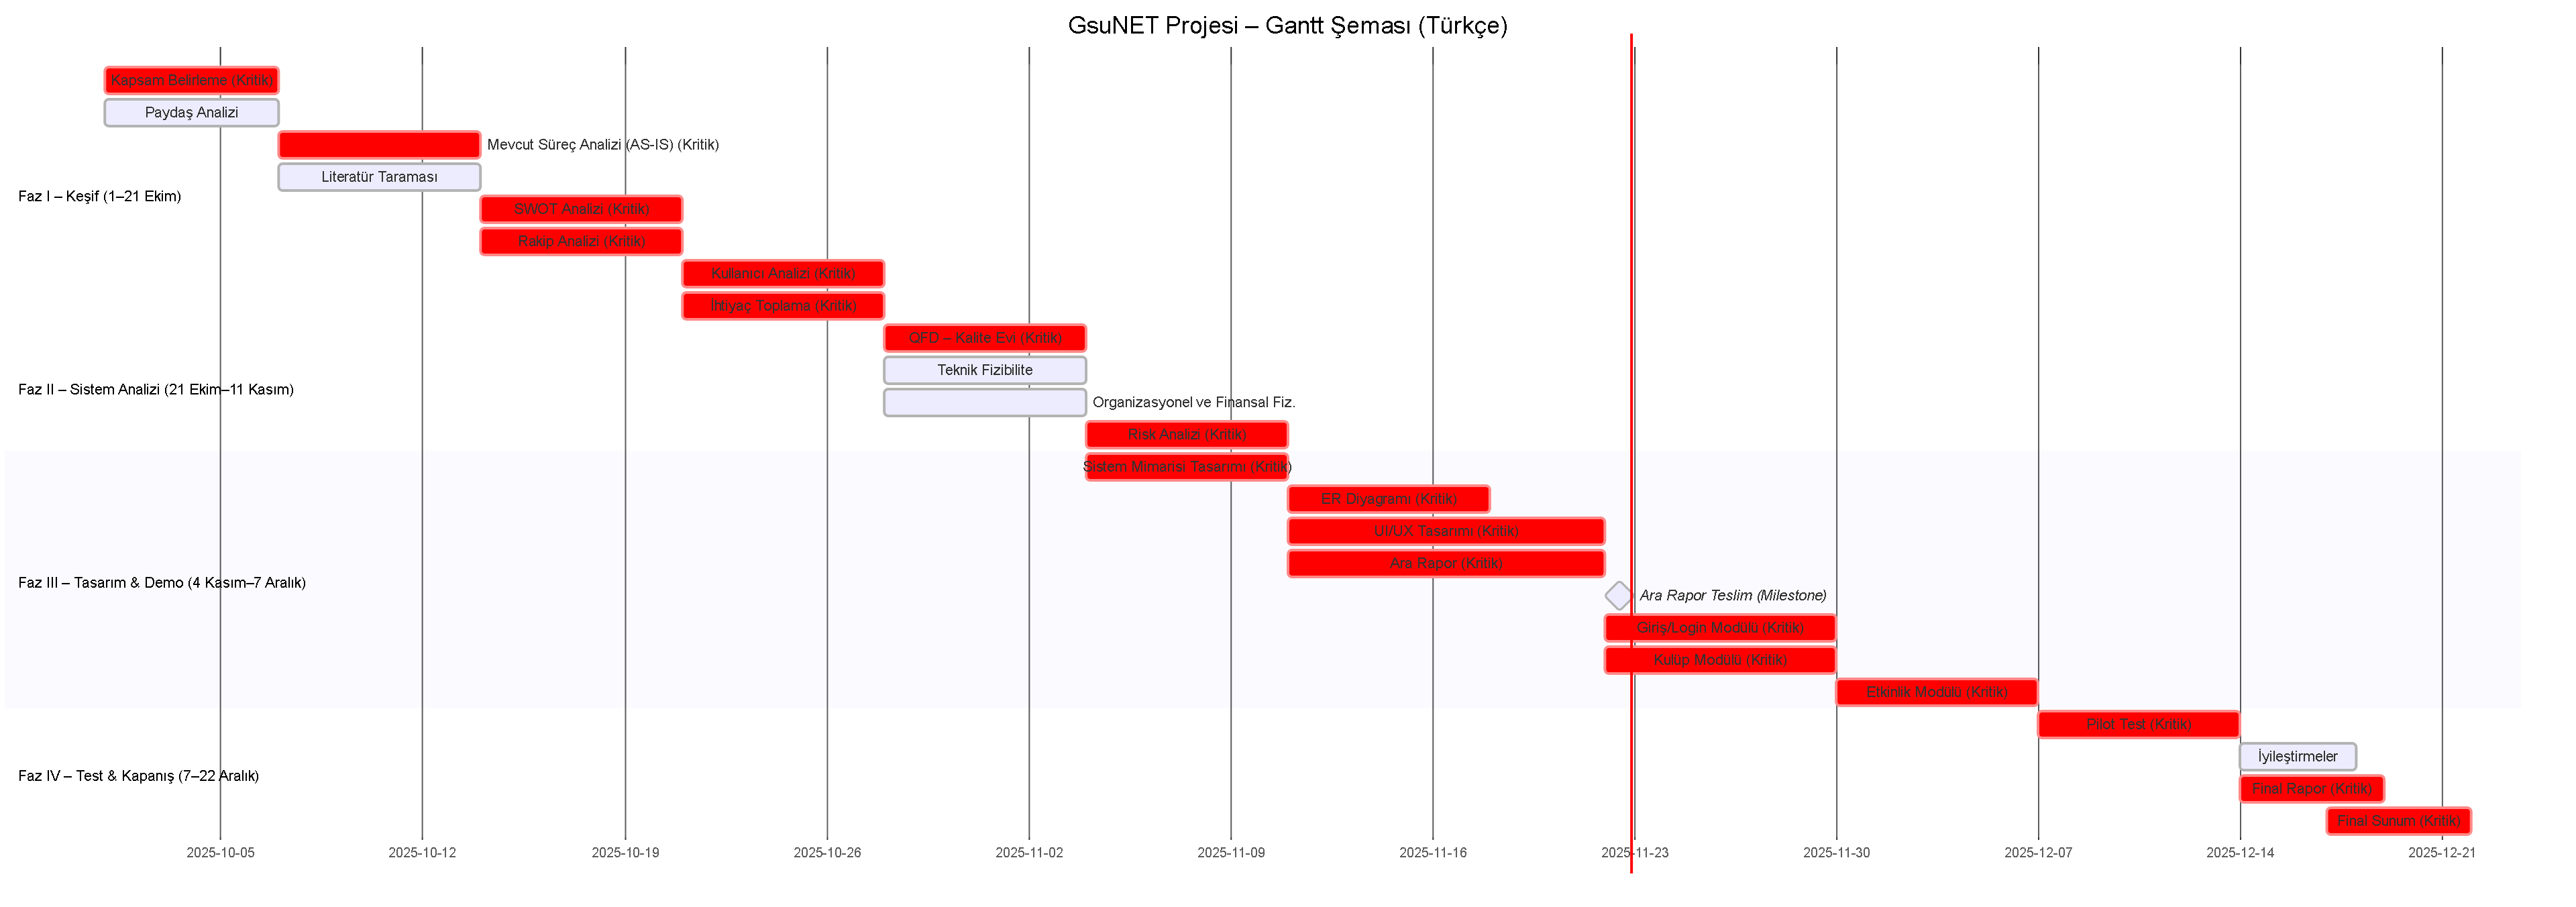
\includegraphics{gantt.png}}
    \caption{GsuNET Proje Zaman Planı (Gantt Şeması)}
    \label{fig:gantt_chart}
\end{figure}


\section{Disiplin Bazlı Görev Dağılımı ve Kritik Yol}

Gantt şemasında görevler; \textbf{Endüstri Mühendisliği odaklı}, \textbf{Bilgisayar Mühendisliği odaklı} ve \textbf{ortak} görevler olarak sınıflandırılmıştır.

\begin{itemize}
    \item \textbf{Endüstri Mühendisliği ağırlıklı görevler:} 2, 3, 4, 5, 6, 7, 8, 9, 10, 11, 12
    \item \textbf{Bilgisayar Mühendisliği ağırlıklı görevler:} 13, 14, 15, 18
    \item \textbf{Ortak görevler:} 1, 16, 17, 19, 20, 21
\end{itemize}

Projenin \textbf{kritik yolu}:

\begin{center}
1 → 3 → 5–6–7 → 8–9 → 12 → 13–14–15 → 16–17 → 18 → 19–20 → 21
\end{center}

Bu zincirde meydana gelebilecek gecikmeler, ara rapor ve final teslim tarihlerini doğrudan etkileyebileceğinden, bu görevler için Gantt şemasında ek tampon süreler kullanılması planlanmıştır.

% --- CPM ŞEMASI GÖRSELİ ---
\begin{figure}[htbp]
    \centering
    % Yüksekliği 10cm yaptık, sığmazsa 12cm veya 8cm yapabilirsin.
    \resizebox{!}{1.2cm}{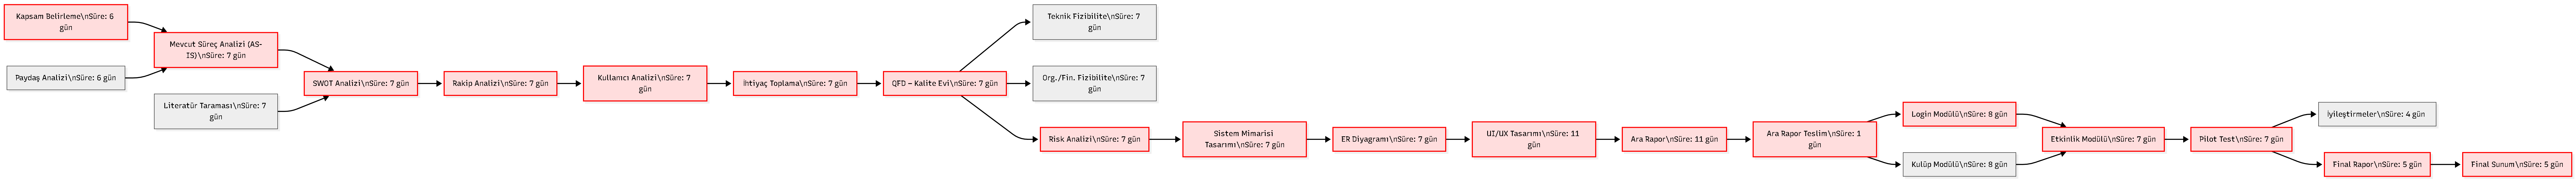
\includegraphics{cpm.png}}
    \caption{Proje Kritik Yol (CPM) Diyagramı}
    \label{fig:cpm_chart}
\end{figure}
% --------------------------

%-----------------------------
\chapter{Sistem Analizi}

\section{Proje ve Problem Tanımı}

Galatasaray Üniversitesi bünyesinde faaliyet gösteren öğrenci kulüpleri, etkinlik ve duyuru süreçlerini günümüzde büyük ölçüde Instagram, WhatsApp, e-posta ve fiziksel afişler gibi dağınık ve sürdürülebilir olmayan kanallar üzerinden yürütmektedir. Bu yöntemler hem duyuruların geniş öğrenci kitlesine ulaşmasını zorlaştırmakta hem de etkinlik görünürlüğünü sınırlamaktadır.

Afişlerin kampüste kısa süre kalabilmesi, bilginin sürekli güncellenememesi, bazı öğrencilerin duyurulara hiç ulaşamaması ve kulüp süreçlerinin manuel yönetilmesi gibi faktörler, kulüplerin hedefledikleri etkileşim seviyesine ulaşmalarını engellemektedir. Buna ek olarak, kulüplerin şirketlerle yürüttüğü sponsorluk görüşmeleri çoğunlukla bireysel bağlantılara dayanmakta; kurumsal ve sistematik bir altyapının olmaması, sponsorlukların sürdürülebilirliğini zayıflatmakta ve üniversite kulüplerinin potansiyel bütçelere erişimini kısıtlamaktadır.

Bu doğrultuda geliştirilen \textbf{GsuNET}, kulüplerin tüm etkinlik, duyuru ve sponsorluk süreçlerini tek bir dijital platformda birleştirerek mevcut dağınıklığı ortadan kaldırmayı ve üniversite çapında bütünleşik bir iletişim ağı oluşturmayı hedeflemektedir. Platform, kulüplerin etkinliklerini daha geniş öğrenci kitlesine ulaşacak şekilde duyurabilmesini, duyuruların dijital olarak saklanmasını ve güncellenmesini, kâğıt-afiş kullanımının azalmasını sağlayarak hem operasyonel verimliliğe hem de sürdürülebilirliğe katkı sunacaktır.

Ayrıca, platform üzerinden şirketlerin kulüplerle doğrudan etkileşime geçebilmesi, sponsorluk taleplerinin standart bir formatta iletilebilmesi ve potansiyel iş birliklerinin artırılması amaçlanmaktadır. Böylece, üniversitenin dış paydaşlar nezdindeki görünürlüğü de güçlenecektir.

GsuNET'in temel hedefleri; \textbf{bilgi akışını merkezi ve erişilebilir hale getirmek}, \textbf{sponsorluk süreçlerini dijitalleştirerek kulüplerin kurumsal ilişkilerini güçlendirmek} ve \textbf{kulüp etkinliklerinin öğrencilere ulaşma oranını artırarak katılımı yükseltmek} olarak tanımlanabilir. Bu bağlamda platformun ana kullanıcı grupları; etkinlikleri takip etmek isteyen öğrenciler, içerik ve süreç yönetiminden sorumlu kulüp yöneticileri ve sponsorluk/etkinlik iş birliklerine ilgi duyan şirketlerdir. GsuNET, bu üç kullanıcı grubunu aynı sistem üzerinde buluşturarak daha görünür, daha ölçülebilir, daha erişilebilir bir kulüp ekosistemi oluşturmayı amaçlamaktadır.

\section{Mevcut Durum Analizi (AS-IS)}

Galatasaray Üniversitesi'nde öğrencilerin ve kulüp topluluklarının yürüttüğü etkinlik, duyuru ve sponsorluk süreçleri günümüzde büyük ölçüde parçalı, manuel ve dijital olarak bütünleşmemiş bir yapı üzerinden işlemektedir. Mevcut durum aşağıdaki alt başlıklarda sistematik şekilde incelenmiştir.

\subsection{Duyuru Süreçlerinin Mevcut Durumu}

GSÜ kulüplerinin etkinlik duyurularını gerçekleştirdiği başlıca kanallar şunlardır:

\begin{itemize}
    \item \textbf{Instagram:} Kulüplerin en aktif kullandığı duyuru aracıdır. Ancak algoritma ve erişim sorunları nedeniyle paylaşımlar tüm öğrencilere ulaşmamaktadır. Duyurular kısa ömürlüdür ve kalıcılığı düşüktür.

    \item \textbf{WhatsApp grupları:} Her bölüm/kulüp kendi grupları içinde duyuru paylaşmaktadır. Ancak bu yapı dağınıktır ve ortak bir erişim alanı oluşmadığı için birçok öğrenci etkinliklerden haberdar olmamaktadır.

    \item \textbf{E-posta:} Bazı kulüpler etkinliklerini e-posta yoluyla duyurmakta; ancak öğrencilerin e-postaları düzenli kontrol etmemesi nedeniyle bu kanal düşük etki yaratmaktadır.

    \item \textbf{Kampüs içi panolar:} Fiziksel panolar aktif kullanılmaktadır; ancak afişler kısa süre kalabilmekte, kalabalık arasında görünürlüğünü kaybedebilmekte ve güncellenebilirliği sınırlıdır.
\end{itemize}

\textbf{Sorun:} Duyurular farklı platformlarda dağınık bir yapıda ilerlediği için öğrencilerin etkinliklere erişimi sınırlanmakta, kulüpler hedefledikleri katılım düzeyine ulaşamamaktadır.

\subsection{Etkinlik Planlama Süreçlerinin Mevcut Durumu}

Etkinliklerin fiziksel olarak gerçekleştirildiği salon ve dersliklerin kullanımıyla ilgili mevcut süreç tamamen manuel ilerlemektedir:

\begin{itemize}
    \item Kulüpler, etkinlik için \textbf{SKS (Sağlık Kültür Spor)} birimine talep iletmektedir.

    \item SKS, ilgili talebi ilgili \textbf{fakülte sekreterliği} ile paylaşarak onay sürecini yürütmektedir.

    \item Tüm süreç e-posta ve bireysel iletişim kanalları üzerinden ilerlediği için takip edilmesi zordur.

    \item Dersliklerin doluluk oranları veya uygunluk bilgileri dijital ortamda görünür değildir.

    \item Bu nedenle kulüpler çoğu zaman \textbf{tahmine dayalı} planlama yapmak zorunda kalmaktadır.
\end{itemize}

\textbf{Sorun:} Salon/derslik uygunluğunun dijital olarak görülememesi, etkinlik planlamasında belirsizlik yaratmakta ve süreç verimliliğini düşürmektedir.

\subsection{Sponsorluk Süreçlerinin Mevcut Durumu}

GSÜ kulüplerinde sponsorluk süreçleri büyük ölçüde \textbf{kişisel bağlantılara} dayalıdır:

\begin{itemize}
    \item Kulüp yöneticileri şirketlere LinkedIn, kişisel e-posta adresleri veya bireysel tanıdıklar aracılığıyla ulaşmaktadır.

    \item Sponsorluk ajansları ile çalışan kulüpler olsa da bu ajanslar genellikle yeterli kapsamda destek sağlayamamaktadır.

    \item Üniversitede sponsorluk başvurusunu standartlaştıran veya şirketlere merkezi şekilde ulaşılmasını sağlayan bir sistem bulunmamaktadır.

    \item Sponsorluk dosyaları, görüşme durumları, olumlu/olumsuz geri dönüşler gibi bilgiler dağınık tutulmaktadır.
\end{itemize}

\textbf{Sorun:} Sponsorluk süreci kurumsal bir çerçeveye sahip olmadığı için kulüpler yüksek potansiyelli iş birliklerine ulaşmakta zorlanmakta ve bütçelerini büyütme imkânı sınırlı kalmaktadır.

\subsection{Kulüpler Arası Koordinasyonun Mevcut Durumu}

Üniversitede çeşitli kulüpler aynı dönemde çok sayıda etkinlik yapmaktadır. Ancak:

\begin{itemize}
    \item Kulüpler arasında ortak bir dijital takvim bulunmamaktadır.

    \item Etkinlik çakışmaları veya benzer kitlelere yönelik aynı gün etkinlik düzenlenmesi sık görülmektedir.

    \item Çoğu kulüp diğer kulüplerin ne zaman, nerede etkinlik yapacağını \textbf{sonradan öğrenmektedir}.
\end{itemize}

\textbf{Sorun:} Koordinasyon eksikliği hem kulüpler hem de öğrenciler için etkileşim kaybına neden olmaktadır.

\subsection{Öğrenci Erişim ve Katılım Süreçleri}

Öğrencilerin kulüpleri ve etkinlikleri takip etme süreci de dijital olarak entegre değildir:

\begin{itemize}
    \item Öğrenciler, ilgilendikleri kulüplerin hesaplarını tek tek takip ederek bilgi almaya çalışmaktadır.

    \item Kulüpler arası farklı iletişim kanalları nedeniyle öğrenciler çoğu etkinliği kaçırmaktadır.

    \item Üniversite genelinde "kişiselleştirilmiş etkinlik akışı" sunan bir sistem bulunmamaktadır.
\end{itemize}

\textbf{Sorun:} Etkinlik bilgilerinin öğrencilere erişimi rastlantısal hâle gelmekte ve öğrenci katılımı düşmektedir.

\subsection{Özet}

Güncel AS-IS analizi, GSÜ kulüplerinin \textbf{duyuru}, \textbf{etkinlik planlama}, \textbf{sponsorluk yönetimi}, \textbf{koordinasyon} ve \textbf{öğrenci erişimi} gibi tüm temel süreçlerde bölük pörçük, manuel ve veriye dayalı olmayan yöntemlerle çalıştığını ortaya koymaktadır. Bu durum, kulüp etkinliklerinin potansiyelini düşürmekte, öğrenci katılımını sınırlamakta ve kurumsal gelişim imkânlarını engellemektedir.

GsuNET projesi, bu mevcut durumu (AS-IS) analiz ederek, tüm süreçleri dijitalleştiren, bütünleştiren ve veri odaklı yöneten bir \textbf{TO-BE (gelecek durum)} yapısına geçişi hedeflemektedir.

\section{SWOT Analizi}

\begin{table}[h]
\centering
\begin{tabular}{|p{7cm}|p{7cm}|}
\hline
\multicolumn{2}{|c|}{\textbf{İÇSEL FAKTÖRLER}} \\
\hline
\textbf{Güçlü Yönler (Strengths)} & \textbf{Zayıf Yönler (Weaknesses)} \\
\hline
\begin{itemize}[leftmargin=*]
    \item Üniversitede farklı ilgi alanlarına hitap eden, aktif bir kulüp ekosistemi bulunması
    \item Öğrencilerin hem akademik hem sosyal etkinliklere katılma isteğinin yüksek olması
    \item Kulüplerin sosyal medya üzerinden içerik üretme ve iletişim kurma konusunda deneyimli olması
\end{itemize}
&
\begin{itemize}[leftmargin=*]
    \item Kulüp, etkinlik ve sponsorluk süreçlerini tek çatı altında toplayan resmi bir dijital platformun bulunmaması
    \item Etkinlik bilgilerinin farklı kanallarda dağınık şekilde paylaşılması ve güncelliğinin takip edilmesindeki zorluklar
    \item Etkinlik katılım, sponsorluk getirisi gibi performans göstergelerinin düzenli ölçülememesi
\end{itemize}
\\
\hline
\multicolumn{2}{|c|}{\textbf{DIŞSAL FAKTÖRLER}} \\
\hline
\textbf{Fırsatlar (Opportunities)} & \textbf{Tehditler (Threats)} \\
\hline
\begin{itemize}[leftmargin=*]
    \item GsuNET'in, üniversitenin dijital dönüşüm vizyonuna katkı sağlayacak pilot bir sistem olarak konumlandırılabilmesi
    \item Sponsorluk süreçlerinin veriye dayalı yönetilmesiyle, kulüplerin kurumsal iş birliklerini güçlendirme potansiyeli
    \item İyi tasarlanmış bir platformun, diğer üniversiteler için de ölçeklenebilir bir model oluşturması
\end{itemize}
&
\begin{itemize}[leftmargin=*]
    \item Öğrencilerin ve kulüp yöneticilerinin alıştıkları iletişim kanallarından vazgeçmek istememesi
    \item Platformun uzun vadeli teknik bakımının ve sahipliğinin net olarak tanımlanmaması durumunda sistemin atıl kalma riski
    \item Veri gizliliği, kişisel verilerin korunması ve yetkisiz erişim gibi bilgi güvenliği riskleri
\end{itemize}
\\
\hline
\end{tabular}
\caption{GsuNET SWOT Analizi}
\end{table}

Bu SWOT analizi, GsuNET'in çözmeyi hedeflediği problem alanlarını ve stratejik konumunu netleştirerek, tasarım ve planlama aşamaları için temel oluşturmuştur.

\section{Pazar ve Rekabet Analizi}

GsuNET platformu, üniversite kulüpleri için çok amaçlı, bütünleşik bir dijital yönetim sistemi sunması nedeniyle hem üniversite içi rakiplerle hem de profesyonel etkinlik platformlarıyla karşılaştırılabilir. Mevcut pazar analizi, GsuNET'in benzersiz değer önerisini ve konumunu ortaya koymak amacıyla iki ana eksende yapılmıştır: (i) Üniversite içi çözümler, (ii) Profesyonel etkinlik ve duyuru platformları.

\subsection{Pazarın Yapısı}

Üniversite ortamında kulüplerin etkinlik, duyuru ve sponsorluk süreçlerini dijital olarak bütünleştiren kapsamlı bir platform bulunmamaktadır. Türkiye'de birçok üniversite sosyal medya ve klasik kurum içi araçlara bağımlı olduğundan pazar, hâlen doygunluktan uzak, açık bir alan olarak konumlanmaktadır. Bu GsuNET için \textbf{"erken konumlanma avantajı"} yaratmaktadır.

Aşağıdaki tablo mevcut pazarın kategorizasyonunu göstermektedir:

\begin{table}[h]
\centering
\small
\begin{tabular}{|p{3cm}|p{3cm}|p{4cm}|p{3.5cm}|}
\hline
\textbf{Pazar Segmenti} & \textbf{Örnekler} & \textbf{Mevcut Durum} & \textbf{GsuNET'e Etkisi} \\
\hline
Üniversite içi duyuru kanalları & Instagram, WhatsApp, e-posta, panolar & Dağınık, sürdürülemez, kısa ömürlü & GsuNET bu alanı tamamen konsolide eder \\
\hline
Üniversite uygulamaları & Özyeğin App, Bilkent Event Paneli & Kısıtlı özellikler, sadece duyuru/etkinlik & GsuNET çok daha geniş kapsamlı \\
\hline
Profesyonel etkinlik platformları & Eventbrite, Biletino, Meetup & Ücretli, topluluk yönetimi yok, üniversite uyumu kısıtlı & Dolaylı rakip; fonksiyon alanları farklı \\
\hline
Sponsorluk yönetim sistemleri & Ajanslar, LinkedIn iletişimi & Bireysel çabalar, süreç bütünleşik değil & GsuNET bu boşluğu doldurur \\
\hline
Üniversite yönetimi birimleri & SKS, fakülte sekreterlikleri & Süreçler manuel, otomasyon yok & GsuNET süreç dijitalleşmesini sağlar \\
\hline
\end{tabular}
\caption{Pazar Segmentasyonu}
\end{table}

\subsection{Rakip Analizi}

Aşağıdaki tablo hem üniversiteler hem de profesyonel platformlar dikkate alınarak hazırlanmış kapsamlı rekabet analizidir (Benchmarking):

\begin{table}[h]
\centering
\tiny
\begin{tabular}{|p{2cm}|p{1.3cm}|p{2cm}|p{1.8cm}|p{2cm}|p{1.8cm}|p{2.5cm}|}
\hline
\textbf{Platform/Üniversite} & \textbf{Duyuru} & \textbf{Etkinlik Yönetimi} & \textbf{Salon/Uygunluk Bilgisi} & \textbf{Sponsorluk Yönetimi} & \textbf{Topluluk Yönetimi} & \textbf{Genel Değerlendirme} \\
\hline
GSÜ (mevcut) & Instagram / Pano & Kısmi & Yok & Yok & Yok & GsuNET'e en uygun ortam \\
\hline
Sabancı & Instagram / Pano & Var & Kısmi & Yok & Yok & Dijital altyapı sınırlı \\
\hline
Koç & Instagram / Pano & Var & Yok & Yok & Yok & Kitle büyük ama çözüm yok \\
\hline
Bilkent Paneli & Var & Kısmi & Yok & Yok & Yok & Sadece duyuru paneli \\
\hline
İTÜ / ODTÜ & Var & Kısmi & Yok & Yok & Yok & Dijital dönüşüm fırsatı \\
\hline
Özyeğin Uygulaması & Var (Okul app'i içinde) & Var & Yok & Yok & Yok & Tek fonksiyonlu, geniş kapsam yok \\
\hline
Eventbrite & Var & Var & Yok & Yok & Yok & Üniversiteye uyumlu değil, ücretli \\
\hline
Meetup & Var & Var & Yok & Yok & Var (topluluk) & Üniversite içi süreçlerle uyumsuz \\
\hline
Biletino & Etkinlik & Biletleme & Yok & Yok & Yok & Sadece etkinlik/katılım odaklı \\
\hline
\textbf{GsuNET} & \textbf{✓ Merkezî} & \textbf{✓ Yönetim + planlama} & \textbf{✓ Dijital görünürlük} & \textbf{✓ Sponsorluk modülü} & \textbf{✓ Topluluk sistemi} & \textbf{En kapsamlı ve uyumlu çözüm} \\
\hline
\end{tabular}
\caption{Rakip Analizi (Benchmarking)}
\end{table}

\subsection{GsuNET'in Rekabet Üstünlüğü (USP – Unique Selling Proposition)}

GsuNET'in rakiplerine kıyasla en önemli üstünlükleri şunlardır:

\begin{itemize}
    \item \textbf{Tüm kulüp süreçlerini tek platformda birleştiren ilk GSÜ sistemi olması} – etkinlik, duyuru, sponsorluk, salon uygunluğu, katılım takibi hepsi bir arada.

    \item \textbf{Üniversite kültürüne özel çözümler sunması} – profesyonel platformların sağlayamadığı "kulüp–SKS–öğrenci" üçgenini dijitalleştirir.

    \item \textbf{Sponsorluk modülü ile kurumsal ilişki yönetimi sağlaması} – benzer üniversitelerde bulunmayan bir özellik.

    \item \textbf{Öğrencilere kişiselleştirilmiş etkinlik akışı sunma kapasitesi} – Instagram'ın rastlantısal erişim sorunlarını ortadan kaldırır.

    \item \textbf{Sürdürülebilirlik katkısı} (kağıt-afiş süreçlerinin minimize edilmesi) – diğer platformlarda yoktur.

    \item \textbf{GSÜ bileşenleri için özgün veri analitiği ve raporlama imkânı} – katılım verisi, kulüp performansı, sponsorluk dönüş oranı vb.
\end{itemize}

\subsection{Rekabetten Kaynaklı Riskler}

\begin{itemize}
    \item Öğrencilerin mevcut alışkanlıklarını (Instagram, WhatsApp) bırakmak istememesi
    \item Profesyonel platformların (Eventbrite, Meetup) işlevsel gücü
    \item GsuNET'in aktif kullanım oranının düşük kalması durumunda değer kaybı
    \item Dijitalleşme sürecinin üniversite birimlerinde zaman alabilmesi
\end{itemize}

Bu riskler, ilerleyen bölümlerde (5.9 Risk Analizi) ayrıntılı şekilde değerlendirilecektir.

\section{Müşteri (Kullanıcı) Analizi}

GsuNET platformunun temel kullanıcı kitlesi üç ana gruptan oluşmaktadır: öğrenciler, kulüp yöneticileri ve şirketler. Bu bölümde kullanıcı grupları, platform üzerindeki ihtiyaç ve davranış biçimleri dikkate alınarak segmentlere ayrılmıştır. Segmentasyon, platformun kullanıcı beklentilerini daha iyi anlamayı, fonksiyonel gereksinimleri netleştirmeyi ve QFD çalışmalarının temelini oluşturmayı amaçlamaktadır.

\subsection{Öğrenci Segmentasyonu (Katılım Sıklığına Göre)}

Öğrenciler etkinliklere katılım seviyelerine göre dört segmentte değerlendirilebilir. Bu segmentasyon, GsuNET'in kullanıcı davranışlarını anlaması ve kişiselleştirilmiş akışlar tasarlaması açısından kritik önemdedir.

\begin{table}[h]
\centering
\small
\begin{tabular}{|p{3cm}|p{5cm}|p{6cm}|}
\hline
\textbf{Segment} & \textbf{Tanım} & \textbf{Davranış \& İhtiyaç Özeti} \\
\hline
Yüksek Katılımcılar (Ayda 3+ etkinlik) & Kulüplerin çoğunu aktif takip eden, düzenli katılım sağlayan öğrenciler & Güncel etkinlik akışı, bildirimler, çakışma takvimi, salon bilgisi, hızlı kayıt \\
\hline
Orta Katılımcılar (Ayda 1–2 etkinlik) & İlgi alanına göre seçici katılım gösteren öğrenciler & Filtrelenmiş etkinlik önerileri, popüler etkinlikler, kişiselleştirilmiş duyurular \\
\hline
Pasif Katılımcılar (Seyrek katılım) & Etkinlikleri sosyal medyada gördükçe katılan öğrenciler & Merkezi duyuru akışı, tekrar eden hatırlatmalar, kolay kayıt \\
\hline
Potansiyel Katılımcılar (Hiç katılmayan) & Etkinliklerden haberdar olmayan veya bilgiye erişimi düşük öğrenciler & Tüm kampüs etkinliklerinin tek ekranda görünmesi, erişilebilirlik, arama fonksiyonları \\
\hline
\end{tabular}
\caption{Öğrenci Segmentleri}
\end{table}

\subsection{Kulüp Yöneticileri Segmentasyonu}

Kulüp yöneticileri GsuNET'in ikinci temel kullanıcı grubudur. İş süreçleri ve operasyonel sorumluluklara göre alt segmentlere ayrılmışlardır.

\begin{table}[h]
\centering
\small
\begin{tabular}{|p{3cm}|p{5cm}|p{6cm}|}
\hline
\textbf{Segment} & \textbf{Tanım} & \textbf{İhtiyaçlar} \\
\hline
Yeni Yönetici & İlk kez kulüp yönetimine katılanlar & Basit arayüz, kullanım rehberi, otomatik duyuru akışı, kolay etkinlik oluşturma \\
\hline
Tecrübeli Yönetici & Daha önce organizasyon yönetmiş kişiler & Gelişmiş planlama, takvim çakışma analizi, salon uygunluğu \\
\hline
Sponsorluk Sorumluları & Şirketlerle iletişim kuran kişiler & Sponsorluk başvuru modülü, şirket profilleri, dönüş takip sistemi \\
\hline
Operasyon Ekipleri & Etkinlik günü süreçlerini yöneten ekip & Kayıt listeleri, QR giriş sistemi, salona özel bilgiler \\
\hline
\end{tabular}
\caption{Kulüp Yöneticisi Segmentleri}
\end{table}

\bigskip
\bigskip
\bigskip
\bigskip
\bigskip
\bigskip
\bigskip
\bigskip
\bigskip
\bigskip


\subsection{Şirket Segmentasyonu}

GsuNET'in üçüncü kullanıcı grubu, kulüplerle sponsorluk iş birlikleri kurmak isteyen şirketlerdir.

\begin{table}[h]
\centering
\small
\begin{tabular}{|p{3.5cm}|p{5cm}|p{5.5cm}|}
\hline
\textbf{Segment} & \textbf{Tanım} & \textbf{Beklentiler} \\
\hline
Büyük Ölçekli Şirketler & Kurumsal sponsorluk stratejisi olan firmalar & Net raporlama, kulüp profili, sponsor paketleri, görünürlük \\
\hline
Startuplar & Hedefli küçük bütçelerle etkinlik yapmayı hedefleyen girişimler & Uygun maliyetli paketler, hızlı iletişim \\
\hline
GSÜ Mezunu Bulunduran Şirketler & GSÜ alumni network etkisiyle iletişim kuran firmalar & Hızlı eşleşme, kulüp geçmiş projeleri \\
\hline
Sponsorluk Ajansları & Kulüpler adına marka yöneten ajanslar & Tek noktadan erişim, etkinlik listeleri, teklif yönetimi \\
\hline
\end{tabular}
\caption{Şirket Segmentleri}
\end{table}

\subsection{Kullanıcı Gruplarının Ortak İhtiyaçları}

\begin{table}[h]
\centering
\small
\begin{tabular}{|p{4cm}|p{10cm}|}
\hline
\textbf{Kullanıcı Grubu} & \textbf{Temel İhtiyaçlar} \\
\hline
Öğrenciler & Merkezi etkinlik akışı, bildirimler, kaos/çakışma olmadan planlama, ilgilerine göre öneri \\
\hline
Kulüp Yöneticileri & Etkinlik oluşturma ve planlama, salon uygunluğu, sponsor yönetimi, raporlama \\
\hline
Şirketler & Kolay iletişim, net kulüp profilleri, sponsor dönüş görünürlüğü, tek kanaldan erişim \\
\hline
\end{tabular}
\caption{Ortak Kullanıcı İhtiyaçları}
\end{table}

Bu segmentasyon, ilerleyen aşamalarda yapılacak personalar, empati haritaları ve Kalite Evi (QFD) çalışmaları için girdileri sağlamaktadır.

\section{Kullanıcı İhtiyaçları (User Needs)}

Bu bölüm, GsuNET platformunun temel kullanıcı gruplarının talep ve beklentilerini sistematik olarak ortaya koymak amacıyla hazırlanmıştır. Kullanıcı ihtiyaçları, platformun fonksiyonel gereksinimlerini ve QFD (Quality Function Deployment) matrisinin girişlerini oluşturacak biçimde derlenmiştir.

Analiz üç ana kullanıcı kitlesi üzerinden yapılmıştır: öğrenciler, kulüp yöneticileri ve şirketler.

\subsection{Öğrenci İhtiyaçları}

\begin{table}[H]
\centering
\small
\begin{tabular}{|p{5cm}|p{9cm}|}
\hline
\textbf{İhtiyaç} & \textbf{Açıklama} \\
\hline
Merkezi etkinlik akışı & Tüm kulüp etkinliklerini tek ekranda, güncel ve sınıflandırılmış olarak görebilme ihtiyacı \\
\hline
Kolay erişim & Sosyal medyaya bağlı kalmadan tüm duyurulara hızlı erişim \\
\hline
Bildirim sistemi & İlgi alanlarına göre anlık hatırlatma ve duyuru iletimi \\
\hline
Etkinlik çakışmalarından kaçınma & Aynı gün gerçekleşen etkinliklerin çakışmadan görüntülenmesi \\
\hline
Etkinlik detaylarının bütünlük içinde sunulması & Tarih, saat, konuşmacı, içerik, yer, kayıt bağlantısı gibi bilgilerin tek yerde olması \\
\hline
Kişiselleştirilmiş öneriler & Katılım geçmişi veya ilgi alanlarına göre etkinlik önerisi alabilme \\
\hline
Kolay kayıt ve katılım & QR kod veya profil üzerinden hızlı etkinlik kaydı \\
\hline
\end{tabular}
\caption{Öğrenci İhtiyaçları}
\end{table}

\subsection{Kulüp Yöneticisi İhtiyaçları}

\begin{table}[H]
\centering
\small
\begin{tabular}{|p{5cm}|p{9cm}|}
\hline
\textbf{İhtiyaç} & \textbf{Açıklama} \\
\hline
Etkinlik oluşturma paneli & Yeni etkinlikleri açıklama, görsel, yer ve saat bilgisi ile birlikte hızlıca oluşturabilme \\
\hline
Salon/derslik uygunluk bilgisi & Etkinlik planlaması için odaların doluluk, saat uygunluğu ve onay takibi \\
\hline
Sponsorluk yönetimi & Şirketlerle iletişim, sponsorluk paketleri ve teklif takip paneli \\
\hline
Duyuruların geniş kitlelere ulaşması & Tek tuşla tüm öğrencilere görünür bir duyuru gönderebilme \\
\hline
Yönetim paneli & Kulüp sayfasını düzenleme, istatistikleri görüntüleme, üye yönetimi \\
\hline
Etkinlik performans raporları & Katılım sayısı, kayıt verisi, geçmiş etkinliklerin analizleri \\
\hline
Operasyonel kolaylık & Etkinlik günü için QR giriş, kayıt listesi, katılım doğrulama araçları \\
\hline
Süreç şeffaflığı & SKS–fakülte onay aşamalarını adım adım takip edebilme \\
\hline
\end{tabular}
\caption{Kulüp Yöneticisi İhtiyaçları}
\end{table}

\subsection{Şirket İhtiyaçları}

\begin{table}[H]
\centering
\small
\begin{tabular}{|p{5cm}|p{9cm}|}
\hline
\textbf{İhtiyaç} & \textbf{Açıklama} \\
\hline
Kulüpler hakkında güvenilir bilgi & Kulübün geçmiş projeleri, kitlesi, etkinlik yapısı, fotoğrafları \\
\hline
Sponsorluk paketlerine erişim & Standartlaştırılmış sponsorluk teklifleri, fiyat aralıkları, görünürlük seviyesi \\
\hline
Kolay iletişim & Tek panel üzerinden ilgili kulüp yetkilisine ulaşabilme \\
\hline
Etkinlik görünürlüğü & Sponsor oldukları etkinliklerin düzenli ve doğru şekilde duyurulması \\
\hline
Performans raporu & Sponsorlu etkinliğin katılım verisi ve geri bildirim analizi \\
\hline
Hızlı dönüş & Sponsorluk taleplerinin bekleme süresinin minimize edilmesi \\
\hline
\end{tabular}
\caption{Şirket İhtiyaçları}
\end{table}

\subsection{Ortak İhtiyaçlar}

\begin{table}[H]
\centering
\small
\begin{tabular}{|p{6cm}|p{8cm}|}
\hline
\textbf{Ortak İhtiyaç} & \textbf{Kullanıcı Grubu} \\
\hline
Doğru, güncel ve merkezi bilgiye erişim & Öğrenciler – Kulüp yöneticileri – Şirketler \\
\hline
Kullanım kolaylığı (kolay arayüz) & Tüm kullanıcılar \\
\hline
Hızlı iletişim ve geri dönüş mekanizması & Kulüp yöneticileri – Şirketler \\
\hline
Güvenilirlik ve veri doğruluğu & Tüm kullanıcılar \\
\hline
Dijital süreç entegrasyonu & Kulüp yöneticileri – Üniversite birimleri \\
\hline
Etkinlik duyurularının görünürlüğü ve erişim gücü & Öğrenciler – Kulüp yöneticileri \\
\hline
Etkinlik performansının ölçülebilir olması & Kulüp yöneticileri – Şirketler \\
\hline
Kurumsal imaj desteği (profesyonel görünüm) & Kulüp yöneticileri – Şirketler \\
\hline
\end{tabular}
\caption{Ortak İhtiyaçlar}
\end{table}

\section{Fizibilite Çalışmaları}

\subsection{Teknik Fizibilite}

GsuNET'in web tabanlı bir platform olarak geliştirilmesi planlanmaktadır. Önerilen teknoloji yığını; modern bir frontend çerçevesi (örneğin React) ve REST tabanlı bir backend (Node.js veya Django) ile ilişkisel bir veritabanı (PostgreSQL vb.) içermektedir. Bu yapı, kullanıcı sayısı ve veri hacmi göz önünde bulundurulduğunda, ölçeklenebilir ve bakımı görece kolay bir çözüm sunmaktadır.

Üniversitenin mevcut bilişim altyapısıyla uyumlu olduğu ve temel güvenlik önlemleri (HTTPS, rol bazlı yetkilendirme, şifrelenmiş veri saklama) ile desteklenebileceği öngörülmektedir.

\subsection{Organizasyonel Fizibilite}

Kulüpler ve danışmanlarla yapılan ön değerlendirmelerde, etkinlik ve duyuruların daha merkezi bir biçimde yönetilmesine yönelik olumlu bir beklenti olduğu gözlemlenmiştir. Platformun sürdürülebilir bir şekilde kullanılabilmesi için:

\begin{itemize}
    \item Dönem başlangıcında kulüp kayıt süreçlerinin GsuNET üzerinden yürütülmesi
    \item Danışman onay mekanizmasının sistemle entegre edilmesi
    \item Üniversite yönetimi tarafından platformun "resmi kulüp yönetim aracı" olarak tanımlanması
\end{itemize}

Bu koşullar sağlandığında, projenin organizasyonel açıdan uygulanabilir olduğu değerlendirilmektedir.

\subsection{Finansal Fizibilite}

Projenin öğrenci projesi olarak geliştirilecek olması, lisanslı yazılım maliyetlerini minimize etmektedir. Açık kaynak teknolojilerin tercih edilmesi durumunda, başlangıçta yalnızca alan adı ve barındırma (hosting) giderleri söz konusu olacaktır.

Küçük ölçekli bir bulut sunucu (veya üniversite sunucuları) ile ilk prototipin barındırılması mümkündür. Uzun vadede, kullanıcı sayısının artması halinde sunucu kapasitesinin yükseltilmesi gerekse de, toplam maliyetin üniversite bütçesi içinde yönetilebilir düzeyde kalacağı öngörülmektedir.

\section{Risk Analizi}

Bu bölümde GsuNET Platformu’nun geliştirme, uygulama ve kullanım aşamalarında ortaya çıkabilecek riskler sistematik olarak değerlendirilmiştir. Her risk; olasılık, etki ve risk skoru üzerinden analiz edilmiş, ardından olasılık–etki matrisine yerleştirilerek risk seviyeleri belirlenmiştir.

\subsection{Risk Tanımları ve Değerlendirme Tablosu}

Aşağıdaki tablo her riskin tanımını, olasılık düzeyini, etkisini, risk skorunu ve uygun azaltım stratejisini göstermektedir.

\begin{table}[H]
\centering
\caption{Risk Değerlendirme Tablosu}
\begin{tabular}{c p{5.2cm} c c c c p{4.5cm}}
\toprule
\textbf{No} & \textbf{Risk Tanımı} & \textbf{Olasılık} & \textbf{Etki} & \textbf{Risk Skoru} & \textbf{Risk Seviyesi} & \textbf{Azaltım Stratejisi} \\
\midrule
R1 & Sunucu performansının yetersiz kalması & 3 & 5 & 15 & Yüksek & Bulut altyapısı, otomatik ölçeklendirme, yük testleri \\
R2 & Bildirim sisteminde gecikme & 4 & 3 & 12 & Orta-Yüksek & Bildirim servislerini mikroservis olarak ayırma \\
R3 & Veritabanında veri tutarsızlığı & 3 & 5 & 15 & Yüksek & Veri bütünlüğü kontrolleri, transaction kullanımı \\
R4 & Kulüplerin platformu geç benimsemesi & 4 & 4 & 16 & Yüksek & Eğitim oturumları, kullanım rehberi, teşvik \\
R5 & Etkinlik bilgilerinin eksik girilmesi & 3 & 3 & 9 & Orta & Zorunlu alanlar, veri doğrulama kuralları \\
R6 & Öğrencilerin platformu yeterince keşfetmemesi & 3 & 4 & 12 & Orta-Yüksek & Basit arayüz, push bildirimleri, tanıtım stratejileri \\
R7 & Güvenlik açığı / yetkisiz erişim & 2 & 5 & 10 & Orta & Rol tabanlı erişim, şifreleme, güvenlik testleri \\
R8 & Mobil uyumluluk kaynaklı kullanım zorluğu & 2 & 4 & 8 & Orta & Responsive tasarım, cihaz bazlı testler \\
R9 & Geliştirme sürecinin gecikmesi & 3 & 4 & 12 & Orta-Yüksek & Faz bazlı geliştirme, kritik yol kontrolü \\
R10 & Sponsorluk modülünün düşük kullanımı & 2 & 3 & 6 & Düşük-Orta & Şirket iletişimi, profil doğrulama, pilot kullanım \\
R11 & Derslik verilerinin SKS'den alınamaması (API eksikliği) & 4 & 3 & 12 & Orta-Yüksek & Dönem başı manuel veri toplama (keşif gezisi), en çok kullanılan dersliklerden önceliklendirme \\
\bottomrule
\end{tabular}
\end{table}

\subsection{Olasılık–Etki Matrisi (Risk Öncelik Matrisi)}

Riskler, olasılık ve etki düzeylerine göre 5×5 matris üzerinde konumlandırılmıştır. Her risk yalnızca bir hücrede yer alır.

\begin{table}[H]
\centering
\caption{Olasılık / Etki Matrisi}
\begin{tabular}{c c c c c c}
\toprule
\textbf{Olasılık →} & \textbf{1} & \textbf{2} & \textbf{3} & \textbf{4} & \textbf{5} \\
\midrule
\textbf{5 – Çok Yüksek} &  &  &  &  & R1, R3 \\
\textbf{4 – Yüksek} &  &  & R2 & R4, R6, R9, R11 &  \\
\textbf{3 – Orta} &  &  & R5 &  &  \\
\textbf{2 – Düşük} &  & R10 & R8 & R7 &  \\
\textbf{1 – Çok Düşük} &  &  &  &  &  \\
\bottomrule
\end{tabular}
\end{table}

\subsection{Risklerin Kategorilere Ayrılması}

\textbf{Yüksek Riskler (kritik müdahale gereken):}
\begin{itemize}
    \item R1 – Sunucu performansı
    \item R3 – Veri tutarsızlığı
    \item R4 – Kulüplerin platforma geç adaptasyonu
\end{itemize}

Bu riskler sistemin çalışabilirliğini veya kullanım yaygınlığını doğrudan etkilediği için geliştirme sürecinde öncelikli olarak ele alınmalıdır.

\textbf{Orta–Yüksek Riskler:}
\begin{itemize}
    \item R2 – Bildirim gecikmesi
    \item R6 – Öğrencilerin platformu keşfetmemesi
    \item R9 – Geliştirme gecikmeleri
    \item R11 – Derslik verilerinin SKS'den alınamaması
\end{itemize}

Bu riskler sistemin kullanım kalitesini ve proje takvimini etkileyebilir; düzenli takip gerektirir.

\textbf{Orta Riskler:}
\begin{itemize}
    \item R5 – Eksik etkinlik verisi
    \item R7 – Güvenlik açığı
    \item R8 – Mobil uyumluluk sorunları
\end{itemize}

\textbf{Düşük–Orta Risk:}
\begin{itemize}
    \item R10 – Sponsorluk modülünün düşük kullanımı
\end{itemize}

\subsection{Azaltım Stratejilerinin Özeti}

\begin{table}[H]
\centering
\caption{Azaltım Stratejisi Özeti}
\begin{tabular}{c p{10cm}}
\toprule
\textbf{Risk Seviyesi} & \textbf{Önerilen Aksiyon} \\
\midrule
Yüksek & Sunucu ölçeklendirme, veri bütünlüğü kontrolleri, kulüp eğitimleri \\
Orta-Yüksek & Basit arayüz, tanıtım, modül ayrıştırma, zaman çizelgesi kontrolü \\
Orta & Veri doğrulama, güvenlik testleri, mobil optimizasyon \\
Düşük & İzleme, pilot kullanım, şirketlerle doğrudan iletişim \\
\bottomrule
\end{tabular}
\end{table}

\subsection{R11 Riski: Veri Entegrasyonu Stratejisi (Detay)}

\textbf{Risk Tanımı:} Üniversite SKS (Ders Kayıt Sistemi) ve Fakülte Sekreterliği'nden derslik kullanım verilerinin dijital ortamda (API veya database erişimi) alınamaması durumu, platformun oda rezervasyon özelliğinin işlevselliğini kısıtlayabilir.

\textbf{Gerçekçi Beklenti:} GSÜ'de geleneksel süreçler (e-posta, manuel talep) hakim olduğundan, kısa vadede SKS'den otomatik veri akışı sağlanması düşük olasılıklıdır. Bu, bürokratik ve teknik altyapı kısıtlarından kaynaklanmaktadır.

\textbf{Azaltım Stratejisi - "Keşif Gezisi" Yaklaşımı:}

Eğer SKS API entegrasyonu sağlanamazsa, aşağıdaki manuel ancak sistematik yöntem uygulanacaktır:

\begin{itemize}
    \item \textbf{Dönem Başı Veri Toplama (İlk Hafta):} Her dönem başında (hafta 1), ekip üyeleri derslik binalarında fiziksel "keşif gezisi" gerçekleştirir. Her dersliğin kapısında asılı olan ders programı fotoğraflanır veya el ile kaydedilir.

    \item \textbf{Önceliklendirme:} Veri girişi, en çok etkinlik yapılan dersliklerden başlatılır (örneğin: H301, H401, H501, KL201 gibi büyük amfiler). Bu sayıde 20-30 kritik derslik ile pilot dönem başlatılabilir.

    \item \textbf{Manuel Veri Girişi:} Toplanan ders programları, yönetici kullanıcılar (admin) tarafından sisteme girilir. Bu işlem dönem başında 1-2 gün içinde tamamlanabilir.

    \item \textbf{Haftalık Güncelleme:} Dönem içinde değişiklikler olursa, kulüp yöneticileri veya sekretaryadan gelen bilgiler üzerinden sistem güncellenebilir.

    \item \textbf{Uzun Vadeli Hedef:} Platformun yaygınlaşması ve pilot başarısı gösterildikten sonra, üniversite yönetimi ile API entegrasyonu için resmi görüşmeler başlatılır. SKS ekibi ile teknik entegrasyon roadmap'i oluşturulur.
\end{itemize}

\textbf{Faydası:} Bu manuel yöntem, projenin tamamen bürokratik sürece bağımlı olmasını önler ve "pilot fazda işler hale getirme" (proof of concept) için yeterli veriyi sağlar. İleride API entegrasyonu sağlandığında, sistem mimarisi zaten hazır olduğundan geçiş sorunsuz yapılabilir.

\subsection{Genel Değerlendirme}

Risk analizi sonucunda platformun karşılaşabileceği kritik risklerin büyük bölümünün teknik altyapı ve kullanıcı adaptasyonu kaynaklı olduğu görülmektedir. Bu risklerin tamamı yönetilebilir düzeydedir ve uygun azaltım stratejileri planlandığında proje uygulanabilirliğini tehdit etmez. Matris sonuçları doğrultusunda özellikle veritabanı bütünlüğü, sunucu performansı ve kullanıcı adaptasyonuna yönelik çalışmalar önceliklendirilmelidir.

\textbf{Özellikle R11 (Veri Entegrasyonu) riski için:} "Keşif gezisi" yaklaşımı, projenin pilot aşamada SKS entegrasyonuna bağımlı olmadan çalışabilir hale gelmesini sağlar. Bu, hem teknik risk azaltımı hem de üniversite yönetimine somut sonuç gösterme (proof of value) açısından kritik öneme sahiptir.


\section{Hedef Kitle Beklentileri ve İhtiyaçları}

Tasarım Odaklı Düşünme yaklaşımı doğrultusunda, kullanıcılarla yapılan görüşmeler ve anketlerden elde edilen bulgular, GsuNET için temel ihtiyaç başlıklarını ortaya koymuştur. Bu ihtiyaçlar, daha sonra Kalite Evi (QFD) ile teknik gereksinimlere dönüştürülecek şekilde yapılandırılmıştır.

Öne çıkan başlıca ihtiyaçlar:

\begin{itemize}
    \item \textbf{Merkezi erişim ihtiyacı:} Öğrenciler, farklı kulüplerin tüm etkinlik bilgilerine tek bir platform üzerinden ulaşmak istemektedir.

    \item \textbf{Şeffaf ve güncel takvim:} Etkinlik tarih, saat, yer ve derslik bilgilerinin güncel, doğru ve çakışmasız biçimde görüntülenmesi istenmektedir.

    \item \textbf{Kişiselleştirilmiş içerik:} Kullanıcılar, ilgi alanlarına uygun kulüp ve etkinlikleri öne çıkaran, gereksiz bilgi yükünü azaltan bir ana sayfa talep etmektedir.

    \item \textbf{Kolay içerik üretimi:} Kulüp yöneticileri, sosyal medyada olduğu kadar hızlı ve esnek biçimde etkinlik postu oluşturmak ve paylaşmak istemektedir.

    \item \textbf{Sponsorluk sürecinin dijitalleştirilmesi:} Kulüpler, sponsorluk taleplerini kaybetmeden takip edebilecekleri, şablonlara dayalı ve kurumsal görünümlü bir yapı beklemektedir.

    \item \textbf{Danışman onayını kolaylaştırma:} Akademisyenler, e-posta trafiğine girmeden, kısa sürede onay verebilecekleri yalın bir arayüz istemektedir.

    \item \textbf{Raporlama ve görünürlük:} Üniversite yönetimi, etkinlik yoğunluğu, katılım oranları ve aktif kulüpler hakkında sayısal verilere ve özet grafiklere ihtiyaç duymaktadır.
\end{itemize}

Bu ihtiyaçlar, QFD matrisinde satırları; sistemin teknik özellikleri ise sütunları oluşturarak, \textbf{"kullanıcı sesi"nin tasarıma doğrudan yansımasını} sağlamaktadır.

\section{Kalite Evi (QFD – House of Quality)}

Bu bölümde, 10 adet müşteri ihtiyacı (WHATs) ile 10 adet teknik gereksinim (HOWs) arasındaki ilişki, \textbf{9–3–1} ağırlıklandırma sistemi kullanılarak değerlendirilmiştir:

\begin{itemize}
    \item \textbf{9 = Çok güçlü ilişki} (siyah daire)
    \item \textbf{3 = Güçlü ilişki} (içi noktalı beyaz daire)
    \item \textbf{1 = Zayıf ilişki} (beyaz üçgen)
\end{itemize}

Her müşteri ihtiyacı için verilen \textbf{önem derecesi}, ilişkisel değerle çarpılarak teknik gereksinimlerin ağırlıklı önem değerleri hesaplanmıştır.

QFD matrisi, kullanıcı sesinin (Voice of Customer) doğrudan sistem tasarımına dönüştürülmesini sağlamaktadır. Matris aracılığıyla:

\begin{itemize}
    \item Hangi teknik gereksinimlerin kullanıcılar için en kritik olduğu belirlenmiştir
    \item Tasarım öncelikleri netleştirilmiştir
    \item Müşteri ihtiyaçları ile teknik çözümler arasında izlenebilir bir bağ kurulmuştur
\end{itemize}

% --- QFD (KALİTE EVİ) GÖRSELİ ---
\begin{figure}[htbp]
    \centering
    \resizebox{12cm}{!}{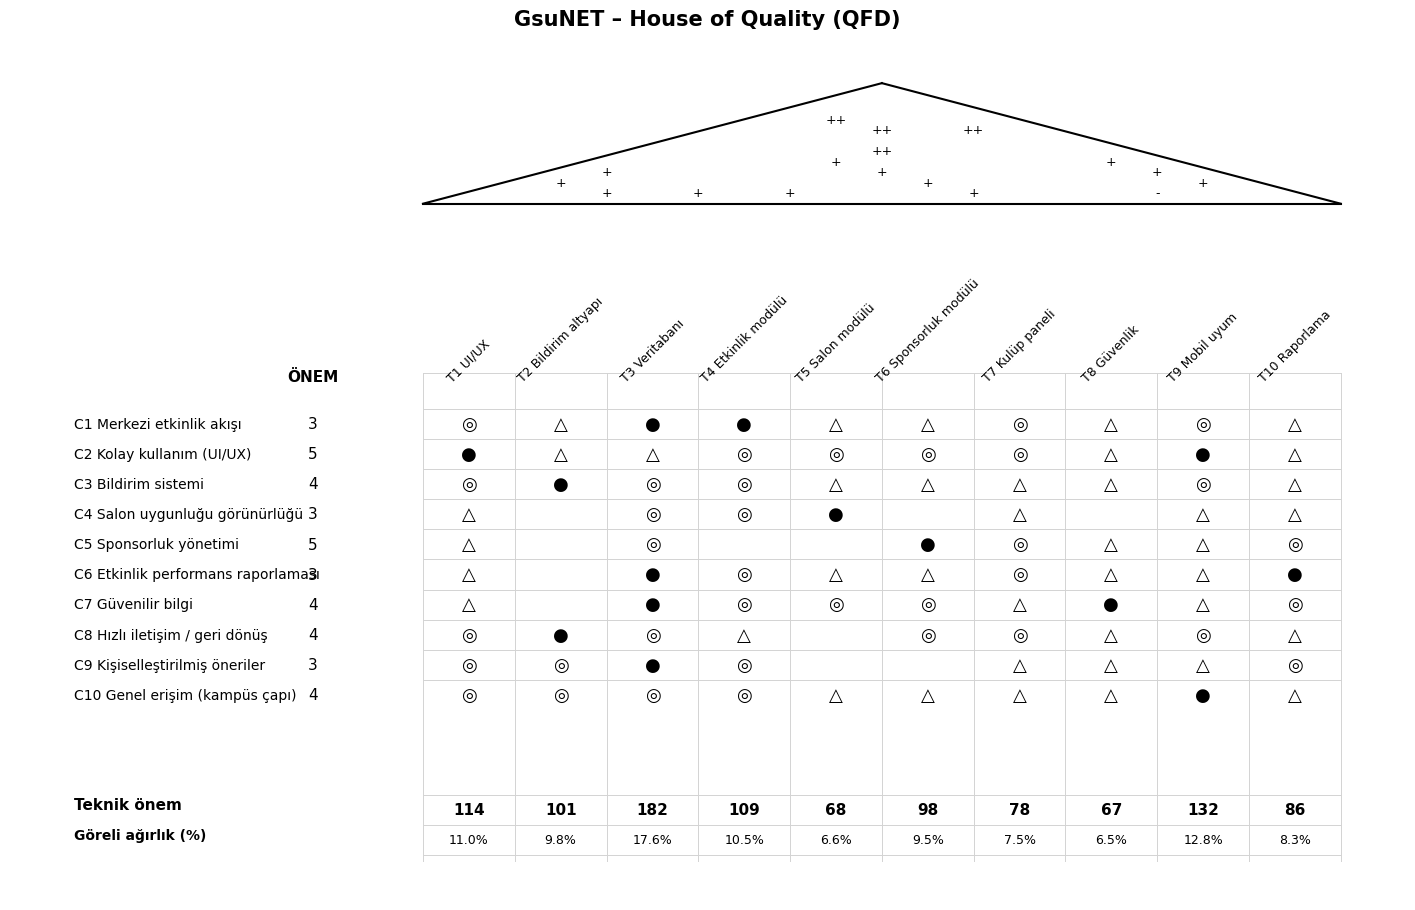
\includegraphics{qfd.png}}
    \caption{GsuNET Kalite Evi (House of Quality) Matrisi}
    \label{fig:qfd_matrix}
\end{figure}
% --------------------------------

Bu yaklaşım, GsuNET'in kullanıcı odaklı bir platform olarak tasarlanmasını güvence altına almaktadır. QFD sonuçları, aşağıdaki bölümlerde detaylandırılmıştır.

\subsection{QFD Sonuçlarının Yorumu}

QFD sonuçlarında en yüksek önceliğin \textbf{veri tabanı altyapısına} verilmesi oldukça tutarlıdır. Çünkü etkinlik akışı, bildirimler, salon uygunluğu, kişiselleştirilmiş öneriler ve güvenilir bilgi gibi tüm temel ihtiyaçlar doğrudan verinin doğru, tutarlı ve hızlı işlenmesine bağlıdır.

\textbf{Mobil uyumluluk ve UI/UX} önemli bir toplam ağırlık oluşturmaktadır. Bu da öğrencilerin platformu yoğun şekilde mobil cihazlardan kullanması nedeniyle tamamen beklenen bir durumdur. Kullanıcı memnuniyeti ve aktif kullanımın devamlılığı bu iki bileşenden geçmektedir.

\textbf{Etkinlik modülü ve bildirim altyapısının} orta-yüksek önem alması, platformun günlük kullanımını tetikleyen ana bileşenler olmalarından kaynaklanmaktadır. Kullanıcıyı sisteme çeken ve sistemde tutan bu modüllerdir.

\textbf{Sponsorluk modülü ve raporlama fonksiyonları} önem sırasında ikinci grupta yer almaktadır. Bu modüller özellikle kulüpler, yöneticiler ve potansiyel sponsorlar için değer yaratmaktadır. Bu yüzden MVP sonrasında geliştirilecek ikinci faz modüller olarak konumlandırılabilirler.

\textbf{Salon uygunluğu modülü ve güvenlik} görece düşük önem yüzdesi almıştır ancak bu düşük önem işlevlerinin önemsiz olduğu anlamına gelmemektedir. Güvenlik kullanıcı tarafından direkt algılanmadığı için düşük puan alabilir; fakat sistem çalışması için zorunludur. Salon modülü ise sadece etkinlik organize eden kulüplerin aktif kullandığı bir özellik olduğu için doğal olarak daha dar bir kitleye hitap etmektedir.

\textbf{Roof (çatı)} kısmındaki korelasyonlar da tasarım sırasında dikkat edilmesi gereken ilişkileri göstermektedir. UI/UX ile mobil uyumluluk arasındaki güçlü pozitif ilişki, tasarımın \textit{mobile-first} yaklaşımını zorunlu kılmaktadır. Veritabanı ile raporlama, güvenlik ve etkinlik modülleri arasındaki yüksek korelasyon, bu modüllerin teknik olarak paralel tasarlanması gerektiğini göstermektedir. Güvenlik ile mobil uyumluluk arasındaki küçük negatif korelasyon ise bazı güvenlik önlemlerinin mobil deneyimi sınırlayabileceğini hatırlatmaktadır; tasarım buna göre optimize edilmelidir.

Genel olarak QFD matrisi, GsuNET'in ilk aşamada kullanıcı deneyimini doğrudan etkileyen modüllere (veritabanı, UI/UX, mobil uyumluluk, etkinlik modülü, bildirimler) ağırlık vermesi gerektiğini; ikinci aşamada ise ekosistemi büyüten modülleri (sponsorluk, raporlama, kulüp paneli) geliştirmesinin doğru olacağını göstermektedir.

\subsection{Teknik Gereksinimlerin Önceliklendirilmesi ve Aksiyon Planı}

QFD matrisi sonuçlarına göre geliştirme sürecinin ilk fazında odaklanılması gereken ana bileşenler: \textbf{Veritabanı yapısı (T3), Mobil uyumluluk (T9), UI/UX (T1), Etkinlik modülü (T4) ve Bildirim altyapısı (T2)} olarak belirlenmiştir. Bu modüller hem kullanıcı deneyimini hem de platformun çalışabilirliğini doğrudan etkilediği için birincil öncelikte ele alınmalıdır.

Veritabanı altyapısının sağlam kurulması, ileride eklenmesi planlanan salon modülü, sponsorluk modülü ve raporlama gibi fonksiyonların sorunsuz entegre edilebilmesini mümkün kılacaktır. Bu nedenle veri modeli, erişim hızları ve bütünlük kontrolleri ilk aşamada tamamlanmalıdır.

Mobil uyumluluk ve UI/UX geliştirmeleri eş zamanlı ilerlemelidir. Öğrencilerin platforma erişim davranışları ağırlıklı olarak mobil üzerinden gerçekleştiği için arayüzün sade, hızlı ve akıcı bir yapıda olması kullanıcı kazanımında kritik rol oynamaktadır.

Etkinlik modülü ve bildirim altyapısı platformun günlük kullanımını artıracak temel bileşenlerdir. Bu iki modülün sorunsuz ve gecikmesiz çalışması hem kulüpler hem de öğrenciler açısından platformun değerini önemli ölçüde artıracaktır.

Orta öncelikli modüller olan \textbf{Sponsorluk modülü (T6), Raporlama (T10) ve Kulüp Paneli (T7)} birincil faz tamamlandıktan sonra geliştirilmelidir. Bu modüller öğrenci deneyiminden çok kulüp operasyonları ve sponsorluk süreci için gerekli olduğundan ikinci fazda ele alınması uygundur.

\textbf{Salon modülü (T5)} ve \textbf{Güvenlik (T8)} düşük öncelikli görünse de sistem işleyişi açısından zorunludur. Bu nedenle temel güvenlik önlemleri ilk fazda sağlanmalı; salon modülü ise MVP kapsamının dışında bırakılabilir ancak ikinci fazda eklenmelidir.

Teknik gereksinimlerin geliştirme sırası, QFD sonuçlarıyla tamamen uyumlu olacak şekilde üç fazda ele alınmalıdır:

\begin{itemize}
    \item \textbf{Faz 1:} T3, T9, T1, T4, T2
    \item \textbf{Faz 2:} T6, T10, T7
    \item \textbf{Faz 3:} T5, T8 (gelişmiş sürümleri)
\end{itemize}

Geliştirme süreci boyunca modüller arasında QFD çatısından gelen korelasyonlara dikkat edilmelidir. Özellikle veri tabanı–raporlama–güvenlik üçlüsü ve UI/UX–mobil uyumluluk ikilisi güçlü ilişkiler gösterdiği için aynı anda planlanmalı veya entegre edilmelidir.

\section{Tasarım Gereksinimleri}

QFD çalışmasının çıktısı olarak, hedef kitle ihtiyaçlarını karşılamak üzere GsuNET için öncelikli tasarım gereksinimleri aşağıdaki gibi tanımlanmıştır:

\subsection{Merkezi Etkinlik Takvimi ve Akış}

Tüm kulüp etkinlikleri, toplantılar ve duyurular tek bir takvimde listelenmeli; kulüp, tarih aralığı ve kategori bazlı filtreleme imkânı bulunmalıdır. Ana sayfada, kullanıcının takip ettiği kulüplere ait içerikler öncelikli olarak gösterilmelidir.

\subsection{Rol Bazlı Erişim ve Yetkilendirme}

Öğrenci, kulüp yöneticisi, akademik danışman ve sistem yöneticisi için farklı arayüzler ve yetki seviyeleri tanımlanmalıdır. Örneğin etkinlik oluşturma yetkisi sadece ilgili kulüp yöneticisinde, onay yetkisi ise danışmanda bulunmalıdır.

\subsection{Derslik ve Kapasite Entegrasyonu}

Etkinlik oluşturma sürecinde, sistem müsait derslikleri ve kapasitelerini sunmalı; çakışan rezervasyonları engellemelidir. Bu amaçla, derslik ve kapasite bilgilerini içeren güncel bir veri tabanı ile entegrasyon sağlanmalıdır.

\subsection{Sponsorluk Yönetim Modülü}

Kulüpler, sponsorluk taleplerini platform üzerinden oluşturabilmeli, teklif şablonları kullanabilmeli ve süreç durumunu (gönderildi, görüşmede, onaylandı, reddedildi vb.) takip edebilmelidir. Sponsorluk lara ilişkin temel finansal bilgiler (sağlanan destek miktarı, türü) kayıt altına alınmalıdır.

\subsection{Bildirim ve Hatırlatma Sistemi}

Yeni etkinlikler, tarih değişiklikleri, danışman onayları ve önemli duyurular için kullanıcıya e-posta ve/veya uygulama içi bildirim gönderilmelidir. Bildirim tercihleri, kullanıcı tarafından yönetilebilir olmalıdır.

\subsection{Veri Toplama ve Raporlama Altyapısı}

Etkinlik başına kayıtlı ve fiili katılım sayıları, kulüplerin yıllık etkinlik sayıları ve sponsorluk hacmi gibi metrikler veri tabanında tutulmalı; grafiksel dashboard'lar üzerinden görüntülenebilmelidir. Bu raporlar, hem kulüp yönetimleri hem de üniversite yönetimi için farklı seviyelerde özetlenebilmelidir.

\subsection{Kullanılabilirlik ve Mobil Uyum}

Arayüz tasarımında sadelik, tutarlılık ve erişilebilirlik ilkeleri gözetilmelidir. Platform, mobil tarayıcılar üzerinden de rahat kullanılabilecek şekilde responsive tasarlanmalıdır.

\bigskip

Bu tasarım gereksinimleri, bir sonraki aşamada hazırlanacak \textbf{mimari tasarım, veri tasarımı ve kullanıcı arayüzleri} bölümlerine doğrudan girdi sağlayacak; böylece sistem analizi ile teknik tasarım arasında izlenebilirlik sağlanacaktır.

\section{Tasarım İlkeleri}

GsuNET’in tasarımı, platformun farklı kullanıcı segmentlerinin gereksinimlerini tek bir bütünleşik yapı içerisinde karşılamayı hedefleyen çok katmanlı bir mimariye sahiptir. Tasarım ilkeleri, hem kullanıcı deneyimini hem de sistemsel sürdürülebilirliği garanti altına alacak prensipler üzerine kurulmuştur.

Aşağıdaki ilkeler, GsuNET’in çekirdek yaklaşımını, teknik mimarisini ve uzun vadeli kullanım stratejisini şekillendirir.

\subsection{Kullanıcı Merkezi Tasarım (User-Centric Design)}

Platformun ana tasarım önceliği, öğrencilerin ve kulüp yöneticilerinin pratik ihtiyaçlarını doğrudan karşılamak üzerine kuruludur. Bu ilke doğrultusunda:

\begin{itemize}
    \item Arayüz tüm segmentler için minimum öğrenme eğrisi gerektirmelidir.
    \item Etkinlik bulma, duyuru takibi, salon uygunluğu gibi temel fonksiyonlar tek adımda erişilebilir olmalıdır.
    \item Karar noktaları kullanıcıyı yormadan, “doğru zamanda doğru bilgi” yaklaşımı ile tasarlanmalıdır.
\end{itemize}

Bu prensip, platformun benimsenme oranı üzerinde doğrudan belirleyici bir etkiye sahiptir.

\subsection{Mobil-Öncelikli Mimari (Mobile-First Approach)}

GSÜ öğrencileri etkinlik duyurularına ve kulüp güncellemelerine ağırlıklı olarak mobil cihazlar üzerinden ulaşmaktadır. Bu nedenle:

\begin{itemize}
    \item GsuNET arayüzü “mobile-first” tasarım paradigmasıyla geliştirilmelidir.
    \item Tüm etkileşimler; ekran boyutu, parmak hareketleri ve okunabilirlik göz önünde bulundurularak optimize edilmelidir.
    \item Bildirim sistemi mobil kullanım senaryolarına göre şekillendirilmelidir.
\end{itemize}

Mobil öncelik, platformun kullanım sıklığını ve erişilebilirliğini artıracak temel ilkedir.

\subsection{Modüler ve Ölçeklenebilir Sistem Yapısı}

Platformun gelişen ihtiyaçlara hızlı uyum sağlayabilmesi için tüm teknik bileşenler modüler şekilde tasarlanmalıdır. Bu anlayış ile:

\begin{itemize}
    \item Etkinlik yönetimi, bildirim altyapısı, sponsorluk modülü, raporlama ve salon görünürlüğü birbirinden bağımsız ama entegre çalışmalıdır.
    \item Veritabanı mimarisi; kapasite artışlarını ve kullanım yoğunluğunu destekleyebilecek şekilde ölçeklenebilir olmalıdır.
    \item Yeni modüller eklenirken mevcut sistemi bozmayan bir kod ve veri yapısı tercih edilmelidir.
\end{itemize}

Bu ilke, GsuNET’in uzun vadeli sürdürülebilirliğini destekler.

\subsection{Tutarlılık ve Basitlik İlkesi}

Platform arayüzünün tüm bölümlerinde ortak bir tasarım dili ve işlem mantığı kullanılmalıdır. Böylece:

\begin{itemize}
    \item Kullanıcı farklı modüllerde farklı davranışlarla karşılaşmaz.
    \item Kulüp yöneticileri ve öğrenciler arayüzü kısa sürede öğrenir.
    \item Süreçler hızlanır ve hata olasılığı düşer.
\end{itemize}

“Basitlik”, burada işlevsellikten ödün vermek anlamına gelmez; aksine karmaşık süreçlerin kullanıcıya en sade hâliyle sunulması anlamına gelir.

\subsection{Veri Güvenilirliği ve Bütünlük}

Etkinlik akışı, salon uygunluğu, sponsorluk bilgileri ve katılım verileri platformun karar mekanizmalarının temelini oluşturur. Bu nedenle:

\begin{itemize}
    \item Tüm veri girişleri doğrulama süreçlerinden geçmelidir.
    \item Kulüplerin veri düzenleme yetkileri kontrollü şekilde tanımlanmalıdır.
    \item Sistem içi veri akışı bütünlük kurallarıyla desteklenmelidir.
\end{itemize}

Bilgi doğruluğu platformun güvenilirliği açısından kritik öneme sahiptir ve üniversite yönetimi için raporlama süreçlerini güçlendirir.

\subsection{Hızlı Geri Bildirim Döngüsü}

Kullanıcıların gerçekleştirdiği her işlem (etkinlik kaydı, duyuru düzenleme, sponsorluk talebi vb.) anlık geri bildirim ile karşılık bulmalıdır:

\begin{itemize}
    \item Başarılı işlem onayı,
    \item Hata mesajı,
    \item Yükleme durumu,
    \item Bildirim teslim bilgisi.
\end{itemize}

Bu döngü kullanıcı deneyimini iyileştirir ve platforma olan güveni artırır.

\subsection{Kurumsal Uyum ve Süreçsel Tutarlılık}

GsuNET, üniversite içi süreçlerle uyumlu çalışmak zorundadır. Bu nedenle sistem tasarımında:

\begin{itemize}
    \item SKS, sekreterlikler ve kulüp danışmanlarının kullandığı resmi süreçler dikkate alınmalıdır.
    \item Etkinlik onay akışları sistem ile paralel kurgulanmalıdır.
    \item Üniversitenin dijitalleşme hedefleriyle uyum sağlanmalıdır.
\end{itemize}

Bu ilke, platformun kurumsal olarak sürdürülebilir olmasını sağlar.

\subsection{Şeffaflık ve İzlenebilirlik}

Platformun tüm kritik işlemleri izlenebilir olmalıdır:

\begin{itemize}
    \item Etkinlik taleplerinin durum geçmişi,
    \item Düzenleme kayıtları,
    \item Sponsorluk görüşme geçmişi,
    \item Kulüp faaliyet takibi.
\end{itemize}

Bu ilke hem kulüpler hem yönetim birimleri için güvenilir bir kullanım alanı sağlar.

\subsection{Genişletilebilir Değer Ekosistemi Tasarımı}

Platform ilerleyen dönemde yeni aktörleri (akademik birimler, mezunlar, organizasyon şirketleri, öğrenci temsilcilikleri) sisteme dahil edebilecek şekilde genişletilebilir olmalıdır.

Bu yaklaşım GsuNET’in yalnızca bir üniversite aracı değil, bir ekosistem platformu olmasını sağlar.

%-----------------------------
\chapter{Sistem Tasarım Araçları ve Yaklaşım}

% 6. Proje konusunun hangi araçlarla sistem tasarımının yapılacağı ve nedenleri
% Teknik analiz – model tasarımı – akış şeması vb.

GsuNET projesinin başarılı bir şekilde tasarlanması ve geliştirilmesi için sistemin farklı katmanlarında çeşitli araçların entegre bir şekilde kullanılması gerekmektedir. Proje ekibimizde yer alan endüstri mühendisliği öğrencileri süreç tasarımı ve analiz araçlarına odaklanırken, bilgisayar mühendisliği öğrencileri teknik tasarım ve geliştirme araçlarından yararlanacaktır. Bu bölümde, projenin sistem tasarımında kullanılacak araçlar ve bu araçların seçilme nedenleri detaylandırılmaktadır.

\section{Sistem Modelleme ve Analiz Araçları}

\subsection{UML (Unified Modeling Language)}

Sistemin genel mimarisini ve bileşenler arası ilişkileri görselleştirmek amacıyla UML diyagramları kullanılacaktır. Özellikle aşağıdaki diyagram türleri tasarım sürecinde önem taşımaktadır:

\begin{itemize}
    \item \textbf{Use Case Diyagramları:} Her kullanıcı grubunun (öğrenci, kulüp yöneticisi, danışman, sponsor) sistemle olan etkileşimlerini tanımlamak için kullanılacaktır. Bu sayede sistemin fonksiyonel gereksinimleri net bir şekilde ortaya konulabilecektir.

    \item \textbf{Class Diyagramları:} Veritabanı yapısının ve nesne yönelimli tasarımın temelini oluşturacaktır. Kulüp, Etkinlik, Kullanıcı gibi ana varlıkların sınıf yapıları ve aralarındaki ilişkiler bu diyagramlarla modellenecektir.

    \item \textbf{Sequence Diyagramları:} Örneğin "bir öğrencinin etkinliğe kayıt olması" veya "sponsor firmanın teklif göndermesi" gibi dinamik süreçlerin adım adım akışını göstermek için kullanılacaktır.

    \item \textbf{Component Diyagramları:} Frontend, backend, veritabanı ve API gateway gibi sistemin temel bileşenlerinin yapısını ve bağımlılıklarını göstermek için tercih edilecektir.
\end{itemize}

UML seçimi, yazılım geliştirme süreçlerinde endüstri standardı olması ve ekip içi iletişimi kolaylaştırması nedeniyle yapılmıştır. Diyagramlar, \textbf{draw.io} veya \textbf{Lucidchart} gibi online araçlar kullanılarak çizilecektir.

\subsection{Entity-Relationship (ER) Diyagramları}

Veritabanı tasarımında varlıklar ve aralarındaki ilişkilerin modellenmesi için ER diyagramları kullanılacaktır. GsuNET platformunda yer alan ana varlıklar (Kullanıcı, Kulüp, Etkinlik, Sponsor, Alan) ve bunlar arasındaki bağlantılar (one-to-many, many-to-many ilişkileri) bu diyagramlarla görselleştirilecektir.

ER diyagramlarının hazırlanmasında \textbf{MySQL Workbench} veya \textbf{dbdiagram.io} gibi araçlar tercih edilecektir. Bu araçlar, hem görsel tasarım hem de SQL script üretimi açısından pratiklik sağlamaktadır.

\section{İş Akışı ve Süreç Tasarım Araçları}

\subsection{Akış Şemaları (Flowcharts)}

Sistemin temel iş akışlarının modellenmesi için akış şemaları kullanılacaktır. Örneğin:

\begin{itemize}
    \item Kulüp yöneticisinin etkinlik oluşturma süreci,
    \item Öğrencinin etkinlik kayıt ve onay akışı,
    \item Sponsor eşleştirme algoritması,
    \item Alan rezervasyon ve çakışma kontrolü.
\end{itemize}

Bu akış şemaları, hem kodlama aşamasında mantık hatalarını önlemek hem de ekip içi anlaşmayı artırmak için kritik öneme sahiptir. Akış şemaları \textbf{Lucidchart} veya \textbf{Microsoft Visio} kullanılarak oluşturulacaktır.

\section{Kullanıcı Arayüzü Tasarım Araçları}

\subsection{Wireframe ve Mockup Araçları}

Kullanıcı arayüzlerinin tasarımı ve prototiplenmesi için \textbf{Figma} platformu kullanılacaktır. Figma, ekip üyeleri arasında gerçek zamanlı işbirliği sağlaması, prototip oluşturma ve kullanıcı testi yapma imkânı sunması nedeniyle tercih edilmiştir.

Figma üzerinde aşağıdaki çalışmalar gerçekleştirilecektir:

\begin{itemize}
    \item Wireframe tasarımları (düşük seviye taslaklar),
    \item High-fidelity mockup'lar (gerçeğe yakın ekran tasarımları),
    \item İnteraktif prototip oluşturma (tıklanabilir demo),
    \item Kullanıcı deneyimi (UX) testleri için materyal hazırlama.
\end{itemize}

\subsection{Kullanıcı Deneyimi (UX) Haritaları}

Kullanıcıların sistem içindeki yolculuklarını (user journey) anlamak ve optimize etmek için \textbf{user flow} ve \textbf{site map} diyagramları hazırlanacaktır. Bu diyagramlar, hangi ekranların hangi sırayla görüntüleneceğini ve kullanıcıların hedeflerine nasıl ulaşacağını gösterecektir.

\section{Veritabanı Tasarım Araçları}

\subsection{İlişkisel Veritabanı Yönetim Sistemi}

GsuNET projesi için \textbf{PostgreSQL 15} veritabanı yönetim sistemi seçilmiştir. Bu seçim, alternatif veritabanı sistemleriyle yapılan detaylı karşılaştırma sonucunda gerçekleştirilmiştir.

\subsubsection{Veritabanı Karşılaştırması}

\begin{table}[h]
\centering
\small
\begin{tabular}{|l|c|c|c|}
\hline
\textbf{Özellik} & \textbf{PostgreSQL 15} & \textbf{MySQL 8.0} & \textbf{MongoDB 7.0} \\ \hline
\textbf{ACID Uyumluluğu} & Tam & Tam & Kısmi \\ \hline
\textbf{JSON Desteği} & JSONB (binary)} & JSON (text) & Natif (BSON) \\ \hline
\textbf{Complex Queries} & Mükemmel & İyi & Zayıf \\ \hline
\textbf{Concurrent Writes} & 10K+ TPS & 8K TPS & 15K TPS \\ \hline
\textbf{Read Performance} & 45K QPS & 40K QPS & 60K QPS \\ \hline
\textbf{Schema Migration} & Alembic/Native & Liquibase & Schemaless \\ \hline
\textbf{Foreign Keys} & Evet & Evet & Hayır \\ \hline
\textbf{Full-Text Search} & Natif (tsquery) & Natif & Atlas Search \\ \hline
\textbf{Lisans} & PostgreSQL (BSD) & GPL/Commercial & SSPL \\ \hline
\end{tabular}
\caption{Veritabanı Performans ve Özellik Karşılaştırması}
\end{table}

\textbf{PostgreSQL'in Seçilme Nedenleri:}

\begin{itemize}
    \item \textbf{Veri Bütünlüğü:} Foreign key constraints, check constraints ve cascade delete özellikleri ile ilişkisel veri modelimizi tam destekliyor.
    \item \textbf{JSONB Performansı:} Room features, notification data gibi semi-structured veriler için binary JSON desteği (\textasciitilde{}30\% daha hızlı).
    \item \textbf{Complex Join Queries:} Kulüp-etkinlik-üye ilişkileri için optimize edilmiş join performansı.
    \item \textbf{Advanced Indexing:} Composite indexes (club\_id + status), GIN indexes (JSONB), B-tree indexes.
    \item \textbf{Timezone-Aware:} Etkinlik tarih/saat yönetimi için \texttt{TIMESTAMP WITH TIME ZONE} desteği.
    \item \textbf{Open Source \& Community:} Geniş topluluk, aktif geliştirme, ücretsiz kullanım.
    \item \textbf{Scalability:} Read replicas, connection pooling (PgBouncer), partitioning desteği.
\end{itemize}

\textbf{MongoDB'a Göre Avantajları:}
\begin{itemize}
    \item Strong schema enforcement (Pydantic + SQLAlchemy)
    \item Transactional consistency (kulüp üyelik onayı + bildirim atomik)
    \item Relational integrity (orphan data prevention)
\end{itemize}

\textbf{Trade-offs:}
\begin{itemize}
    \item MongoDB'a göre daha yavaş write performance (10K vs 15K TPS) - GSUNET için yeterli.
    \item Schema migration complexity (Alembic) - düzenli release cycle ile yönetilebilir.
\end{itemize}

Veritabanı tasarımında \textbf{normalizasyon} prensipleri uygulanacak, veri tekrarı minimize edilecek ve sorgu performansı composite indexes ile optimize edilecektir.

\section{Backend ve API Tasarım Araçları}

\subsection{RESTful API Tasarımı}

Sistemin frontend ve backend katmanları arasındaki iletişim için \textbf{RESTful API} mimarisi kullanılacaktır. API endpoint'lerinin tasarımı ve dokümantasyonu için \textbf{Swagger/OpenAPI} standartları benimsenecektir.

Swagger, API'lerin otomatik dokümantasyonunu sağlaması ve interaktif test ortamı sunması nedeniyle tercih edilmiştir. Bu sayede, frontend ve backend ekipleri arasındaki koordinasyon kolaylaşacaktır.

\subsection{Backend Framework Seçimi}

Ara rapor aşamasında backend geliştirme için \textbf{Django (Python)} veya \textbf{Express.js (Node.js)} frameworkleri değerlendirilmişti. Ancak detaylı teknik analiz ve performans gereksinimleri göz önünde bulundurularak \textbf{FastAPI (Python 3.12)} tercih edilmiştir.

\subsubsection{Framework Karşılaştırması ve Seçim Gerekçesi}

FastAPI'nin seçilmesindeki temel faktörler aşağıdaki karşılaştırmalı analize dayanmaktadır:

\begin{table}[h]
\centering
\small
\begin{tabular}{|l|c|c|c|}
\hline
\textbf{Metrik} & \textbf{FastAPI} & \textbf{Django} & \textbf{Flask} \\ \hline
\textbf{Throughput (req/s)} & 18,000 & 3,000 & 2,500 \\ \hline
\textbf{Response Time (ms)} & 55 & 240 & 280 \\ \hline
\textbf{Async/Await Desteği} & Natif & Kısmi (3.1+) & Eklenti \\ \hline
\textbf{API Dokümantasyon} & Otomatik (OpenAPI) & Manuel & Eklenti \\ \hline
\textbf{Type Safety} & Pydantic & Kısmi & Yok \\ \hline
\textbf{Öğrenme Eğrisi} & Orta & Yüksek & Düşük \\ \hline
\textbf{Performans Skoru} & 9.5/10 & 6/10 & 5.5/10 \\ \hline
\end{tabular}
\caption{Backend Framework Performans Karşılaştırması (TechEmpower Benchmarks Round 22)}
\end{table}

\textbf{FastAPI'nin Seçilme Nedenleri:}

\begin{itemize}
    \item \textbf{Yüksek Performans:} Django'ya göre \textbf{6 kat} daha hızlı istek işleme kapasitesi (18K vs 3K req/s).
    \item \textbf{Asenkron Mimari:} Natif async/await desteği ile ARQ background worker entegrasyonu sorunsuz.
    \item \textbf{Otomatik Dokümantasyon:} OpenAPI/Swagger entegrasyonu ile \texttt{/docs} endpoint'i otomatik oluşturuluyor.
    \item \textbf{Type Safety:} Pydantic ile runtime validation ve IDE auto-completion desteği.
    \item \textbf{Modern Python:} Python 3.12+ özellikleri (type hints, dataclasses) tam destek.
    \item \textbf{Düşük Latency:} Ortalama 55ms response time ile real-time notification sistemine uygun.
\end{itemize}

\textbf{Trade-offs:}

\begin{itemize}
    \item Django'nun admin panel'i gibi hazır özellikler yok (özel AdminPanel.jsx geliştirildi).
    \item Express.js'e göre daha az JavaScript ekosistem uyumluluğu (Python ekosistemi tercih edildi).
    \item Flask'a göre daha fazla boilerplate kod (type safety karşılığında kabul edilebilir).
\end{itemize}

Bu karşılaştırmalı analiz sonucunda FastAPI, GSUNET'in yüksek performans ve ölçeklenebilirlik gereksinimlerini en iyi karşılayan framework olarak seçilmiştir.

\section{Frontend Geliştirme Araçları}

\subsection{Modern JavaScript Framework'leri}

Kullanıcı arayüzünün geliştirilmesi için \textbf{React.js} veya \textbf{Vue.js} gibi modern JavaScript framework'leri kullanılacaktır. Bu framework'lerin seçilme nedenleri:

\begin{itemize}
    \item Component-based yapı (tekrar kullanılabilir bileşenler),
    \item Dinamik ve reaktif kullanıcı arayüzleri oluşturma imkânı,
    \item Geniş topluluk desteği ve zengin kütüphane ekosistemi,
    \item Mobil uyumlu (responsive) tasarım kolaylığı.
\end{itemize}

\subsection{CSS Framework ve Tasarım Sistemi}

Kullanıcı arayüzünün tutarlı ve estetik olması için \textbf{Tailwind CSS} veya \textbf{Material-UI} gibi CSS framework'leri kullanılacaktır. Bu araçlar, tasarım sistemi oluşturmayı kolaylaştırmakta ve geliştirme sürecini hızlandırmaktadır.

\section{Versiyon Kontrol ve İşbirliği Araçları}

\subsection{Git ve GitHub}

Proje kodunun versiyon kontrolü ve ekip işbirliği için \textbf{Git} ve \textbf{GitHub} kullanılacaktır. GitHub üzerinde:

\begin{itemize}
    \item Kod değişikliklerinin takibi (commit history),
    \item Branch stratejisi ile paralel geliştirme (feature branches),
    \item Pull request ve code review süreçleri,
    \item Issue tracking ile görev yönetimi.
\end{itemize}

\subsection{Kullanıcı Kabul Testleri (UAT)}

Sistemin gerçek kullanıcılar tarafından test edilmesi için pilot kullanıcı grupları oluşturulacak ve geri bildirimler toplanacaktır. Bu aşamada \textbf{Google Forms} veya \textbf{Typeform} ile anketler düzenlenecektir.

\section{Dokümantasyon Araçları}

Proje süresince oluşturulan tüm teknik dokümantasyon ve raporlar için \textbf{LaTeX} kullanılacaktır (bu rapor gibi). Kod dokümantasyonu için ise \textbf{JSDoc} (JavaScript) veya \textbf{Sphinx} (Python) gibi otomatik dokümantasyon araçları tercih edilecektir.

\bigskip

Sonuç olarak, GsuNET projesinin sistem tasarımı çok katmanlı bir araç setiyle desteklenmektedir. Her bir araç, belirli bir ihtiyaca yönelik olarak seçilmiş olup ekip üyeleri arasında iş bölümünü kolaylaştırmakta ve projenin başarılı bir şekilde tamamlanmasına katkı sağlamaktadır.

%-----------------------------
\chapter{Veri Seti}

\section{Veri Setinin Belirlenmesi}

GsuNET platformunun etkin bir şekilde çalışabilmesi için, sistemde kullanılacak verilerin kapsamının ve kaynağının doğru şekilde tanımlanması gerekmektedir. Projenin yapısı gereği, hem öğrenci kulüplerine hem de genel üniversite topluluğuna ait çeşitli veri tiplerinin bütünleşik bir ortamda toplanması, saklanması ve işlenmesi temel bir gerekliliktir. Bu nedenle proje kapsamında kullanılacak veri seti, işlevsel gereksinimlere göre aşağıdaki ana veri gruplarından oluşmaktadır.

\subsection{Kullanıcı Verileri}

Sistem üzerinde işlem yapacak tüm kullanıcılar için temel profil verilerinin saklanması zorunludur. Bu veri seti şu bileşenleri içerir:

\begin{itemize}
    \item Öğrenci, danışman ve akademisyen kimlik bilgileri (ad, soyad, öğrenci numarası, rol),
    \item Kullanıcı giriş bilgileri ve yetkilendirme seviyeleri,
    \item Kullanıcının takip ettiği kulüpler ve etkinlik geçmişi,
    \item Bildirim tercihleri ve kişisel takvim entegrasyonu kayıtları.
\end{itemize}

Bu veriler, kullanıcı deneyimini kişiselleştirmek ve sistemdeki erişim kontrollerini düzenlemek için kullanılacaktır.

\subsection{Kulüp ve Organizasyon Verileri}

GsuNET’in merkezinde yer alan öğrenci kulüpleri için bir yönetim ve arşivleme altyapısı oluşturulacaktır. Bu kapsamda ihtiyaç duyulan veri bileşenleri şunlardır:

\begin{itemize}
    \item Kulüp kimlik bilgileri (kulüp adı, açıklama, misyon),
    \item Yönetim kurulu bilgileri ve görev dağılımları,
    \item Kulüp üyeleri ve üyelik statüleri,
    \item Kulübe ait geçmiş ve planlanan etkinlik kayıtları,
    \item Toplantı notları, katılımcı listeleri ve karar dökümleri.
\end{itemize}

Bu veri seti, kulüplerin kurumsal hafızasını dijital ortamda sürdürülebilir kılmayı amaçlamaktadır.

\subsection{Etkinlik ve Duyuru Verileri}

Etkinlikler, GsuNET sisteminin en yoğun veri üreten bileşenidir. Bu kapsamda tutulması gereken veri alanları şunlardır:

\begin{itemize}
    \item Etkinlik adı, açıklaması, tarih ve saat bilgileri,
    \item Etkinliğe ait görseller ve duyuru materyalleri,
    \item Kapasite bilgisi, kontenjan durumu ve kayıt listeleri,
    \item Etkinlik sponsorluk bilgileri,
    \item Etkinlik kategorisi ve hedef kitle segmentasyonu.
\end{itemize}

Bu veriler, öğrencilerin etkinliklere kayıt olmasını, kulüp yönetimlerinin etkinlik süreçlerini takip etmesini ve sponsorların etkinlik verilerini analiz etmesini sağlar.

\subsection{Alan ve Kapasite Yönetimi Verileri}

Üniversite bünyesindeki fiziksel alanların doğru planlanabilmesi için aşağıdaki bilgilerin sistemde bulunması gerekmektedir:

\begin{itemize}
    \item Tüm derslik ve amfilerin kapasite bilgileri,
    \item Rezervasyon takvimi ve uygunluk durumları,
    \item Alan kullanım geçmişi ve çakışma analizleri.
\end{itemize}

Bu veri seti, etkinliklerin uygun mekânlarda planlanabilmesi için gereklidir.

\subsection{Sponsorluk ve Kurumsal İletişim Verileri}

Sponsorluk süreçlerinin dijital platforma entegre edilebilmesi için proje kapsamında şu veriler toplanacaktır:

\begin{itemize}
    \item Sponsor firma profilleri,
    \item Sponsorluk talepleri, teklifler ve görüşme kayıtları,
    \item Sponsorluk geçmişi ve kulüp eşleşmeleri.
\end{itemize}

Bu veri seti, sponsor–kulüp ilişkisinin sürdürülebilir ve izlenebilir olmasını destekleyecektir.

\subsection{Veri Kaynakları ve Toplama Yöntemleri}

GsuNET sisteminde kullanılacak veriler aşağıdaki kaynaklardan temin edilecektir:

\begin{itemize}
    \item Üniversite öğrenci bilgi sistemi (öğrenci kimlik ve rol verileri),
    \item Kulüp yönetimlerinin sağladığı organizasyon ve üyelik verileri,
    \item Kullanıcıların sistem üzerinden gerçekleştirdiği kayıt ve takip işlemleri,
    \item Üniversite yönetimi tarafından sağlanan derslik ve kapasite bilgileri,
    \item Sponsor firmalar tarafından sisteme girilen profil ve teklif verileri.
\end{itemize}

Bu veriler, sistemde kullanılmadan önce güvenlik, doğruluk, gizlilik ve tutarlılık açısından kontrol edilecek; gereksinim duyulan alanlarda anonimleştirme ve veri bütünlüğü denetimleri uygulanacaktır.

\bigskip

Sonuç olarak, GsuNET’in sağlıklı bir şekilde çalışabilmesi için çok katmanlı ve dinamik bir veri setine ihtiyaç vardır. Bu veri seti, platformun tüm kullanıcı gruplarına değer üretmesini sağlayacak altyapıyı oluşturacak ve hem organizasyonel hem de teknik süreçlerin temelini oluşturacaktır.


%-----------------------------
\chapter{Sistem Tasarımı ve Arayüzler}

\section{Genel Sistem Mimarisi}

GSUNET, modern web uygulamaları için yaygın olarak kullanılan \textbf{üç katmanlı mimari} (three-tier architecture) yapısını benimsemektedir. Bu mimari yaklaşım, sistemin ölçeklenebilirliğini, bakım yapılabilirliğini ve güvenliğini artırmak amacıyla tasarlanmıştır.

\subsection{Sunum Katmanı (Presentation Layer)}

Kullanıcıların sistem ile etkileşimde bulunduğu katmandır. React.js framework'ü kullanılarak geliştirilmiş olan bu katman, responsive (duyarlı) tasarım prensipleri ile tüm cihazlarda sorunsuz çalışabilecek şekilde tasarlanmıştır.

\begin{itemize}
    \item \textbf{Teknoloji:} React 19.x, Vite, TailwindCSS
    \item \textbf{Özellikler:} Single Page Application (SPA), komponent tabanlı mimari, state yönetimi
    \item \textbf{Responsive Tasarım:} Desktop ve mobil cihazlar için optimize edilmiş arayüzler
\end{itemize}

\subsection{İş Mantığı Katmanı (Business Logic Layer)}

Sistemin tüm iş kurallarının ve veri işleme mantığının yer aldığı katmandır. FastAPI framework'ü kullanılarak Python dilinde geliştirilmiştir.

\begin{itemize}
    \item \textbf{Teknoloji:} FastAPI, Python 3.12, Pydantic
    \item \textbf{Özellikler:} RESTful API, asenkron işlem desteği, otomatik API dokümantasyonu
    \item \textbf{Güvenlik:} JWT tabanlı kimlik doğrulama, rol bazlı erişim kontrolü
\end{itemize}

\subsection{Veri Katmanı (Data Layer)}

Sistemin tüm verilerinin saklandığı ve yönetildiği katmandır. İlişkisel veritabanı modeli kullanılmaktadır.

\begin{itemize}
    \item \textbf{Teknoloji:} PostgreSQL 15, SQLAlchemy ORM
    \item \textbf{Cache ve Queue:} Redis, ARQ (Async Redis Queue)
    \item \textbf{Özellikler:} ACID uyumlu işlemler, veri bütünlüğü, indeksleme
\end{itemize}

\subsection{Arka Plan İşlem Katmanı (Background Processing Layer)}

Zaman alıcı işlemlerin asenkron olarak yürütüldüğü katmandır.

\begin{itemize}
    \item \textbf{Teknoloji:} ARQ Worker, Redis
    \item \textbf{Kullanım Alanları:}
    \begin{itemize}
        \item Toplu bildirim gönderimi
        \item Etkinlik hatırlatıcıları (cron job, günlük saat 09:00)
        \item Otomatik etkinlik tamamlama
    \end{itemize}
\end{itemize}

\section{Modül ve Bileşenler}

GSUNET sistemi, işlevsel bağımsızlık ve yüksek kohezyon prensiplerine uygun olarak modüler bir yapıda geliştirilmiştir.

\subsection{Kimlik Doğrulama ve Yetkilendirme Modülü}

\textbf{Amaç:} Kullanıcıların sisteme güvenli bir şekilde giriş yapmalarını ve rol bazlı erişim kontrolünü sağlamak.

\textbf{Bileşenler:}
\begin{itemize}
    \item Kullanıcı kaydı ve doğrulama
    \item JWT token üretimi ve doğrulama
    \item Şifre sıfırlama işlemleri
    \item Rol bazlı yetkilendirme (Student, Club Manager, Advisor, Admin)
\end{itemize}

\textbf{Girdi/Çıktı:}
\begin{itemize}
    \item Girdi: E-posta, şifre, kullanıcı bilgileri
    \item Çıktı: JWT access token, kullanıcı profili
\end{itemize}

\subsection{Etkinlik Yönetim Modülü}

\textbf{Amaç:} Etkinliklerin oluşturulması, onaylanması, düzenlenmesi ve takip edilmesi süreçlerini yönetmek.

\textbf{Bileşenler:}
\begin{itemize}
    \item Etkinlik oluşturma ve düzenleme
    \item Onay süreci yönetimi
    \item Oda tavsiye sistemi (kapasite bazlı)
    \item Etkinlik kayıt ve katılımcı yönetimi
    \item Otomatik etkinlik tamamlama (geçmiş etkinlikler)
\end{itemize}

\textbf{Girdi/Çıktı:}
\begin{itemize}
    \item Girdi: Etkinlik bilgileri, tarih/saat, kapasite, oda seçimi
    \item Çıktı: Etkinlik nesnesi, onay durumu, katılımcı listesi
\end{itemize}

\subsection{Kulüp Yönetim Modülü}

\textbf{Amaç:} Öğrenci kulüplerinin dijital yönetimini sağlamak.

\textbf{Bileşenler:}
\begin{itemize}
    \item Kulüp profili yönetimi
    \item Üyelik talepleri ve onay süreci
    \item Kulüp takip sistemi (follow/unfollow)
    \item Kulüp etkinlikleri görüntüleme
\end{itemize}

\textbf{Girdi/Çıktı:}
\begin{itemize}
    \item Girdi: Kulüp bilgileri, üyelik talepleri
    \item Çıktı: Kulüp profili, üye listesi, etkinlik geçmişi
\end{itemize}

\subsection{Oda ve Program Yönetim Modülü}

\textbf{Amaç:} Üniversite odalarının ve haftalık ders programının yönetimi.

\textbf{Bileşenler:}
\begin{itemize}
    \item Oda tanımları ve kapasite bilgileri
    \item Haftalık tekrarlayan program blokları (dersler)
    \item Tek seferlik program blokları (etkinlikler)
    \item Haftalık program görünümü (7 gün)
    \item Oda çakışma kontrolü
\end{itemize}

\textbf{Girdi/Çıktı:}
\begin{itemize}
    \item Girdi: Oda bilgileri, program bloğu detayları, tarih aralığı
    \item Çıktı: Oda listesi, haftalık program, uygunluk durumu
\end{itemize}

\subsection{Bildirim Yönetim Modülü}

\textbf{Amaç:} Kullanıcıların sistem içindeki olaylardan haberdar edilmesini sağlamak.

\textbf{Bileşenler:}
\begin{itemize}
    \item Bildirim oluşturma (senkron ve asenkron)
    \item Bildirim tipleri (etkinlik onayı, iptal, hatırlatıcı, kulüp güncellemeleri)
    \item Toplu bildirim gönderimi (background task)
    \item Bildirim okuma/silme işlemleri
\end{itemize}

\textbf{Girdi/Çıktı:}
\begin{itemize}
    \item Girdi: Bildirim tipi, mesaj, hedef kullanıcılar
    \item Çıktı: Bildirim nesnesi, okunma durumu
\end{itemize}

\subsection{Arka Plan İşlem Modülü}

\textbf{Amaç:} Zaman alıcı işlemlerin HTTP isteklerini bloke etmeden asenkron olarak çalıştırılması.

\textbf{Bileşenler:}
\begin{itemize}
    \item ARQ Worker sistemi
    \item Etkinlik iptal bildirimleri (queue)
    \item Etkinlik hatırlatıcıları (cron job - günlük 09:00)
    \item Toplu bildirim görevleri
\end{itemize}

\textbf{Girdi/Çıktı:}
\begin{itemize}
    \item Girdi: Görev parametreleri (etkinlik ID, kullanıcı listeleri)
    \item Çıktı: Görev sonucu, işlem logları
\end{itemize}

\section{Kullanıcı Arayüzleri (Demo)}

GSUNET'in kullanıcı arayüzleri, modern ve kullanıcı dostu bir deneyim sunmak amacıyla tasarlanmıştır. Arayüzler, farklı kullanıcı rollerine göre özelleştirilmiş içerik ve işlevsellik sunmaktadır.

\subsection{Giriş ve Kayıt Ekranları}

\textbf{Login Sayfası:}
\begin{itemize}
    \item E-posta ve şifre ile giriş
    \item "Şifremi Unuttum" linki
    \item Dil seçimi (Türkçe, İngilizce, Fransızca)
    \item Responsive tasarım ile mobil uyumlu
\end{itemize}

\textbf{Kayıt Sayfası:}
\begin{itemize}
    \item Detaylı form validasyonu
    \item Şifre güvenlik gereksinimleri göstergesi
    \item Öğrenci numarası, bölüm ve tam ad bilgileri
    \item Otomatik hoş geldin bildirimi
\end{itemize}

\subsection{Ana Sayfa (Events Dashboard)}

\textbf{Özellikler:}
\begin{itemize}
    \item Tüm etkinliklerin listelenmesi
    \item Durum bazlı filtreleme (Onaylandı, Beklemede, Reddedildi, İptal, Tamamlandı)
    \item Etkinlik kartlarında:
    \begin{itemize}
        \item Etkinlik başlığı ve açıklaması
        \item Tarih, saat ve lokasyon bilgisi
        \item Kapasite ve kayıt durumu
        \item "Kayıt Ol" butonu
    \end{itemize}
    \item Responsive grid layout
\end{itemize}

\subsection{Kulüpler Sayfası}

\textbf{Özellikler:}
\begin{itemize}
    \item Tüm kulüplerin grid görünümü
    \item "Tüm Kulüpler" ve "Takip Ettiklerim" sekmeleri
    \item Kulüp kartlarında:
    \begin{itemize}
        \item Kulüp adı ve açıklaması
        \item Üye ve takipçi sayısı
        \item "Takip Et" / "Takibi Bırak" butonları
    \end{itemize}
    \item Kulüp detay sayfası:
    \begin{itemize}
        \item Kulüp bilgileri
        \item Kulüp etkinlikleri
        \item Üye listesi
        \item "Katılım Talebi Gönder" butonu
    \end{itemize}
\end{itemize}

\subsection{Etkinliklerim Sayfası}

\textbf{Özellikler:}
\begin{itemize}
    \item Kullanıcının kayıtlı olduğu etkinliklerin listesi
    \item Etkinlik kartları ile detaylı görünüm
    \item Kayıt sayısı göstergesi
    \item "Kaydı İptal Et" seçeneği
\end{itemize}

\subsection{Bildirimler Sayfası}

\textbf{Özellikler:}
\begin{itemize}
    \item Tüm bildirimler listesi
    \item Filtreleme: Tümü, Okunmamış, Okunmuş
    \item "Tümünü Okundu İşaretle" butonu
    \item "Okunanları Sil" butonu
    \item Bildirim tipleri:
    \begin{itemize}
        \item Etkinlik onaylandı
        \item Etkinlik reddedildi
        \item Etkinlik iptal edildi
        \item Etkinlik hatırlatıcısı (3 gün önceden)
        \item Kulüp güncellemeleri
    \end{itemize}
\end{itemize}

\subsection{Kulüp Yönetimi Sayfası (Club Manager)}

\textbf{Özellikler:}
\begin{itemize}
    \item Yönetilen kulüp bilgileri
    \item "Yeni Etkinlik Oluştur" butonu
    \item Katılım talepleri:
    \begin{itemize}
        \item Bekleyen talepler
        \item Onaylama/reddetme butonları
    \end{itemize}
    \item Kulüp açıklaması düzenleme
    \item Üye listesi ve yönetimi
\end{itemize}

\subsection{Etkinlik Oluşturma Sayfası}

\textbf{Özellikler:}
\begin{itemize}
    \item Kapsamlı form validasyonu
    \item Oda tavsiye sistemi (kapasite bazlı)
    \item Kapasite kontrolü:
    \begin{itemize}
        \item Beklenen kapasite \textless= Maksimum kapasite
        \item Gerçek zamanlı uyarı gösterimi
    \end{itemize}
    \item Süre hesaplaması (dakika cinsinden)
    \item Üye-sadece etkinlik seçeneği
    \item Otomatik lokasyon doldurma (oda seçimi ile)
\end{itemize}

\subsection{Onay Paneli (Advisor)}

\textbf{Özellikler:}
\begin{itemize}
    \item Bekleyen etkinlikler sekmesi
    \item Reddedilen etkinlikler sekmesi
    \item Etkinlik detayları:
    \begin{itemize}
        \item Tüm etkinlik bilgileri
        \item Kulüp bilgisi
        \item Kapasite ve lokasyon
    \end{itemize}
    \item "Onayla" ve "Reddet" butonları
    \item Red sebebi girişi (zorunlu)
\end{itemize}

\subsection{Admin Panel}

\textbf{Kullanıcı Yönetimi:}
\begin{itemize}
    \item Tüm kullanıcıların listesi
    \item Filtreleme:
    \begin{itemize}
        \item Rol bazlı filtreleme
        \item İsim bazlı arama
        \item Öğrenci numarası bazlı arama
    \end{itemize}
    \item Kullanıcı rolü değiştirme
    \item Kullanıcı silme
    \item Pagination (10 kullanıcı/sayfa)
\end{itemize}

\textbf{Kulüp Yönetimi:}
\begin{itemize}
    \item Yeni kulüp oluşturma
    \item Kulüp düzenleme
    \item Manager ve Advisor atama
\end{itemize}

\textbf{Program Yönetimi:}
\begin{itemize}
    \item Haftalık program görünümü (Pazartesi-Pazar)
    \item Hafta navigasyonu (Önceki/Mevcut/Sonraki Hafta)
    \item Tekrarlayan program blokları (dersler)
    \item Tek seferlik bloklar (etkinlikler)
    \item Program bloğu ekleme/silme
    \item Filtreleme:
    \begin{itemize}
        \item Oda bazlı filtreleme
        \item Gün bazlı filtreleme
    \end{itemize}
    \item Pagination (10 blok/sayfa)
    \item Legend (Açıklama): Tekrarlayan Ders / Etkinlik (Tek Seferlik)
\end{itemize}

\textbf{Oda Yönetimi:}
\begin{itemize}
    \item Oda listesi
    \item Yeni oda ekleme
    \item Oda bilgileri: İsim, kapasite, açıklama
    \item Pagination (10 oda/sayfa)
\end{itemize}

\subsection{Mobil Navigasyon}

\textbf{Özellikler:}
\begin{itemize}
    \item Alt navbar (bottom navigation)
    \item Responsive tasarım (mobil/desktop geçişi)
    \item Admin için özel mobil menü:
    \begin{itemize}
        \item Modal açılır menü
        \item 4 admin bölümü (Kullanıcılar, Kulüpler, Program, Odalar)
    \end{itemize}
    \item Dil değiştirici (üst navbar)
    \item Bildirim zili (okunmamış sayısı göstergesi)
\end{itemize}

\subsection{Çoklu Dil Desteği}

GSUNET, 3 dilde tam destek sunmaktadır:
\begin{itemize}
    \item \textbf{Türkçe (TR):} Ana dil
    \item \textbf{İngilizce (EN):} İkinci dil
    \item \textbf{Fransızca (FR):} Üçüncü dil
\end{itemize}

Tüm arayüz metinleri, form etiketleri, buton isimleri ve bildirimler dinamik olarak seçilen dilde gösterilmektedir.

\section{Ölçeklenebilirlik Analizi (Scalability)}

GSUNET, üniversite genelinde on binlerce kullanıcıya hizmet verebilecek şekilde tasarlanmıştır. Sistemin ölçeklenebilirlik stratejisi, hem dikey (vertical) hem de yatay (horizontal) scaling yaklaşımlarını desteklemektedir.

\subsection{Message Queue/Task Queue Karşılaştırması}

Background job processing için teknoloji seçimi kritik öneme sahiptir:

\begin{table}[h]
\centering
\small
\begin{tabular}{|l|c|c|c|}
\hline
\textbf{Özellik} & \textbf{Redis + ARQ} & \textbf{RabbitMQ} & \textbf{Kafka} \\ \hline
\textbf{Throughput (msg/s)} & 100,000 & 20,000 & 1,000,000+ \\ \hline
\textbf{Latency (ortalama)} & <1ms & \textasciitilde{}5ms & \textasciitilde{}10ms \\ \hline
\textbf{Kullanım Amacı} & Simple queue & Traditional MQ & Event streaming \\ \hline
\textbf{Complexity} & Düşük & Orta & Yüksek \\ \hline
\textbf{Memory Usage} & In-memory & Disk-backed & Disk-backed \\ \hline
\textbf{Python Integration} & ARQ (async) & Celery/Pika & kafka-python \\ \hline
\textbf{Cron Jobs} & Natif (ARQ) & Plugin & Eklenti \\ \hline
\textbf{Setup Time} & <5 dakika & \textasciitilde{}30 dakika & \textasciitilde{}2 saat \\ \hline
\end{tabular}
\caption{Message Queue Karşılaştırması}
\end{table}

\textbf{Redis + ARQ Seçimi:}

\begin{itemize}
    \item \textbf{Basitlik:} Tek Redis instance ile hem cache hem queue.
    \item \textbf{Düşük Latency:} <1ms ile real-time notifications için ideal.
    \item \textbf{FastAPI Uyumluluğu:} Async Python ile seamless entegrasyon.
    \item \textbf{Yeterli Throughput:} 100K msg/s GSUNET için fazlasıyla yeterli.
    \item \textbf{Cron Job Desteği:} Günlük etkinlik hatırlatıcıları için natif.
\end{itemize}

\textbf{Kafka'ya Göre:} GSUNET event streaming değil simple task queue gerektiriyor. Kafka'nın complexity'si gerekmez (over-engineering).

\textbf{RabbitMQ'ya Göre:} Daha hızlı (5x), daha basit setup, FastAPI async ile daha iyi uyumlu.

\subsection{Horizontal Scaling Stratejisi}

\begin{table}[h]
\centering
\small
\begin{tabular}{|l|c|c|c|}
\hline
\textbf{Kullanıcı Sayısı} & \textbf{FastAPI Instances} & \textbf{PostgreSQL} & \textbf{Redis} \\ \hline
\textbf{1,000 (GSÜ pilot)} & 1 instance & 1 primary & 1 instance \\ \hline
\textbf{10,000 (full GSÜ)} & 2-3 instances & 1 primary + 1 read replica & 1 instance \\ \hline
\textbf{50,000 (multi-uni)} & 8-10 instances & 1 primary + 3 replicas & Redis Cluster (3 nodes) \\ \hline
\textbf{100,000+ (national)} & 15-20 instances & Partitioned DB & Redis Cluster (6 nodes) \\ \hline
\end{tabular}
\caption{Kullanıcı Sayısına Göre Scaling Planı}
\end{table}

\textbf{Load Balancer Mimarisi:}

\begin{itemize}
    \item \textbf{Frontend:} Nginx reverse proxy (round-robin load balancing)
    \item \textbf{Backend:} Multiple FastAPI instances + Uvicorn workers (4 worker/instance)
    \item \textbf{Database:} PgBouncer connection pooling + PostgreSQL streaming replication
    \item \textbf{Redis:} Redis Sentinel (high availability) + Redis Cluster (sharding)
\end{itemize}

\textbf{Performans Tahminleri:}

\begin{itemize}
    \item \textbf{Concurrent Users:} 10K (peak), avg response time <100ms
    \item \textbf{Events per Day:} \textasciitilde{}50-100 (GSÜ scale)
    \item \textbf{Notifications:} 10K bulk notifications <5 seconds (ARQ background)
    \item \textbf{Database Queries:} 1K QPS (current), 45K QPS max capacity
\end{itemize}

\subsection{Caching Stratejisi}

\begin{itemize}
    \item \textbf{Event Listesi:} 5 dakika TTL (sık değişmeyen)
    \item \textbf{Club Bilgileri:} 10 dakika TTL
    \item \textbf{User Sessions:} 7 gün TTL (JWT token ile sync)
    \item \textbf{Room Schedule:} 1 saat TTL (haftalık program nadiren değişir)
\end{itemize}

\subsection{Multi-Tenant Architecture (Çoklu Üniversite Desteği)}

GSUNET'in en önemli ölçeklenebilirlik avantajlarından biri, \textbf{multi-tenant mimarisi} sayesinde birden fazla üniversiteye aynı altyapı üzerinden hizmet verebilme kapasitesidir.

\subsubsection{Mimari Tasarım}

\textbf{Tenant Isolation Strategy:}

\begin{itemize}
    \item \textbf{Database Level:} Her üniversite için ayrı \texttt{university\_id} kolonu (tüm tablolarda foreign key).
    \item \textbf{Query Filtering:} SQLAlchemy ORM ile otomatik tenant filtering (middleware-based).
    \item \textbf{Data Isolation:} Bir üniversitenin kullanıcıları diğer üniversitelerin verilerine erişemez.
    \item \textbf{Shared Infrastructure:} Tek PostgreSQL instance, tenant-based partitioning.
\end{itemize}

\textbf{Tenant Management:}

\begin{itemize}
    \item Her üniversite için \texttt{University} tablosu:
    \begin{itemize}
        \item \texttt{subdomain} - gsu.gsunet.com, boun.gsunet.com, itu.gsunet.com
        \item \texttt{name} - Galatasaray Üniversitesi, Boğaziçi Üniversitesi, ...
        \item \texttt{tier} - Free, Premium, Enterprise (SaaS model)
        \item \texttt{max\_users}, \texttt{max\_clubs}, \texttt{max\_events} (limit kontrolü)
    \end{itemize}
    \item Frontend: Subdomain-based routing → Backend tenant detection (JWT claim)
    \item Admin Super Panel: Tüm üniversiteleri yönetebilme (yeni tenant ekleme, ayarlar)
\end{itemize}

\subsubsection{Ölçeklenebilirlik Senaryoları}

\textbf{Senaryo 1: Galatasaray Üniversitesi (Pilot)}
\begin{itemize}
    \item \textbf{Kullanıcı:} 1,000-2,000 (öğrenci + yöneticiler)
    \item \textbf{Altyapı:} 1 FastAPI instance, 1 PostgreSQL, 1 Redis
    \item \textbf{Maliyet:} \textasciitilde{}₺2,000/ay (2 vCPU, 4GB RAM server)
\end{itemize}

\textbf{Senaryo 2: 5 Üniversite (Regional Expansion)}
\begin{itemize}
    \item \textbf{Kullanıcı:} 10,000-15,000 total
    \item \textbf{Tenant Sayısı:} GSÜ, Boğaziçi, İTÜ, ODTÜ, Koç (5 tenant)
    \item \textbf{Altyapı:} 4 FastAPI instances (Nginx load balancer), PostgreSQL master + 2 read replicas, Redis Cluster (3 nodes)
    \item \textbf{Maliyet:} \textasciitilde{}₺15,000/ay (8 vCPU, 32GB RAM total)
    \item \textbf{Gelir:} 5 üniversite × ₺75,000/yıl = ₺375K/yıl → Net: ₺195K/yıl
\end{itemize}

\textbf{Senaryo 3: 20+ Üniversite (National Scale)}
\begin{itemize}
    \item \textbf{Kullanıcı:} 50,000-100,000 total
    \item \textbf{Tenant Sayısı:} 20-30 üniversite (Türkiye'de 200+ devlet/özel üniversite var)
    \item \textbf{Altyapı:}
    \begin{itemize}
        \item 15-20 FastAPI instances (Kubernetes auto-scaling)
        \item PostgreSQL partitioning (tenant-based sharding)
        \item Redis Cluster (6 nodes, 64GB total memory)
        \item CDN (CloudFlare) for static assets
    \end{itemize}
    \item \textbf{Maliyet:} \textasciitilde{}₺45,000/ay (cloud infrastructure)
    \item \textbf{Gelir:} 20 üniversite × ₺75,000/yıl = ₺1.5M/yıl → Net: ₺960K/yıl
\end{itemize}

\subsubsection{Teknik Avantajlar}

\begin{table}[h]
\centering
\small
\begin{tabular}{|l|p{10cm}|}
\hline
\textbf{Avantaj} & \textbf{Açıklama} \\ \hline
\textbf{Cost Efficiency} & Shared infrastructure → her üniversite için ayrı sunucu gerekmez. 20 üniversite tek cluster'da çalışabilir. \\ \hline
\textbf{Instant Deployment} & Yeni üniversite \textasciitilde{}5 dakikada eklenebilir (yeni database seed, subdomain config). \\ \hline
\textbf{Centralized Updates} & Bir update tüm tenantlara aynı anda deploy edilir (zero-downtime rolling update). \\ \hline
\textbf{Data Privacy} & Her tenant'ın verisi izole, cross-tenant data leak imkansız (middleware + ORM filtering). \\ \hline
\textbf{Scalability} & Yeni tenant eklemek horizontal scaling gerektirmez, mevcut infra yeterli (100K user'a kadar). \\ \hline
\textbf{SaaS Model} & Freemium/Premium tier sistemi (small universities free, large universities pay). \\ \hline
\end{tabular}
\caption{Multi-Tenant Architecture Avantajları}
\end{table}

\textbf{Sonuç:} GSUNET, sadece Galatasaray Üniversitesi için değil, \textbf{tüm Türkiye üniversiteleri için SaaS platformu} olarak ölçeklenebilir. Mevcut mimari, 100K+ kullanıcıyı destekleyecek şekilde tasarlanmıştır.

\section{Akıllı Sponsor Eşleştirme Sistemi (AI-Powered)}

GSUNET'in yenilikçi özelliklerinden biri, yapay zeka destekli sponsor-kulüp eşleştirme sistemidir. Bu sistem, sponsorların manifestoları ile kulüplerin profillerini otomatik olarak analiz ederek en uygun eşleşmeleri önerir.

\subsection{Sistem Mimarisi}

\textbf{Akış:}
\begin{enumerate}
    \item Sponsor manifestosunu sisteme yükler (şirket değerleri, hedef kitle, bütçe, sponsorluk tercihleri).
    \item Backend, tüm aktif kulüplerin verilerini toplar:
    \begin{itemize}
        \item Kulüp adı, açıklaması, kategori
        \item Geçmiş etkinlik bilgileri (başlık, katılımcı sayısı, tarihler)
        \item Kulüp sponsorluk tercihleri (finansal, malzeme, etkinlik desteği)
        \item Üye sayısı, takipçi sayısı
    \end{itemize}
    \item Manifesto + kulüp verileri → AI modeline gönderilir.
    \item AI, semantic matching ile en uygun 3-5 kulübü önerir.
    \item Sonuçlar hem sponsor hem de kulüplere bildirim olarak iletilir.
\end{enumerate}

\subsection{AI Model Seçimi ve Karşılaştırma}

\begin{table}[h]
\centering
\small
\begin{tabular}{|l|c|c|c|}
\hline
\textbf{Model} & \textbf{Gemma 7B} & \textbf{Llama 3 (8B)} & \textbf{ChatGPT-4o-mini} \\ \hline
\textbf{Deployment} & Local (GPU) & Local (GPU) & API (Cloud) \\ \hline
\textbf{Cost} & Ücretsiz & Ücretsiz & \$0.15 / 1M tokens \\ \hline
\textbf{Latency} & 50-70ms & 70-100ms & 200-300ms \\ \hline
\textbf{Türkçe Desteği} & İyi & Mükemmel & Mükemmel \\ \hline
\textbf{Semantic Match} & 7/10 & 8.5/10 & 9.5/10 \\ \hline
\textbf{Setup Complexity} & Yüksek (GPU) & Yüksek (GPU) & Düşük (API key) \\ \hline
\textbf{Scalability} & Sınırlı (GPU) & Sınırlı (GPU) & Unlimited \\ \hline
\end{tabular}
\caption{AI Model Karşılaştırması}
\end{table}

\textbf{Seçim Stratejisi:}

\begin{itemize}
    \item \textbf{Demo/Pilot:} ChatGPT-4o-mini API (hızlı entegrasyon, demo kredisi)
    \item \textbf{Production (Low Budget):} Gemma 7B local deployment (ücretsiz, privacy)
    \item \textbf{Production (High Volume):} ChatGPT-4o API (en iyi quality, sınırsız scale)
\end{itemize}

\textbf{Seçim Gerekçesi (Demo):}

ChatGPT-4o-mini API tercih edildi çünkü:
\begin{itemize}
    \item \textbf{Hızlı Entegrasyon:} API key ile 10 dakikada hazır.
    \item \textbf{Demo Kredisi:} OpenAI \$5 ücretsiz kredi (demo için yeterli).
    \item \textbf{Türkçe Performansı:} GPT-4 ailesi Türkçe'de en iyi semantic understanding.
    \item \textbf{Zero Infrastructure:} GPU server kurulumu gerekmez.
\end{itemize}

\textbf{Future Work:}

Production'da maliyet optimizasyonu için:
\begin{itemize}
    \item Fine-tuned Gemma 7B (kulüp-sponsor eşleştirme dataset'i ile)
    \item Hybrid approach: Basit eşleştirmeler için vector similarity, karmaşık için ChatGPT API
\end{itemize}

\subsection{Prompt Engineering}

\textbf{Example Prompt:}

\begin{verbatim}
Sen bir sponsor-kulüp eşleştirme uzmanısın.
Sponsor Manifestosu: {manifesto}
Kulüp Bilgileri: {club_data}

Görev: Bu sponsor için en uygun 3 kulübü seç ve her
biri için eşleşme nedenini açıkla (100-150 kelime).

Format:
1. [Kulüp Adı] (Skor: X/10)
   - Neden: ...
   - Ortak Değerler: ...
   - Potansiyel Projeler: ...
\end{verbatim}

\subsection{Cold Start Problem ve Fall-back Mekanizması}

\textbf{Problem Tanımı:} AI-powered sponsor eşleştirme sisteminin semantic matching yapabilmesi için yeterli veri (kulüp geçmişi, etkinlik detayları, katılımcı demografisi) gerekir. Ancak platformun ilk lansmanında kulüplerin bu düzeyde veri zenginliği olmayabilir. Bu durum "cold start problem" olarak bilinir.

\textbf{Senaryolar:}

\begin{enumerate}
    \item \textbf{Yeni Kulüp (Minimal Data):} Az sayıda etkinlik, sınırlı açıklama, sponsor geçmişi yok.
    \item \textbf{Yeni Platform (Bootstrap Phase):} Hiçbir kulübün henüz yeterli veri birikimi yok.
    \item \textbf{Yeni Sponsor (No Context):} İlk kez platform kullanıyor, hangi kulüplerle eşleşebileceği belirsiz.
\end{enumerate}

\textbf{Fall-back Mekanizması (3-Tier Approach):}

\textbf{Tier 1: Minimal Data (Keyword Matching)}

Eğer kulüp profili sadece ad ve kısa açıklama içeriyorsa:
\begin{itemize}
    \item \textbf{Basit TF-IDF veya Keyword Extraction:} Sponsor manifestosundaki anahtar kelimeler ile kulüp açıklamasındaki kelimeler karşılaştırılır.
    \item \textbf{Category-based Filtering:} Kulüp kategorisi (Spor, Sanat, Teknoloji, Sosyal) ile sponsor hedef kitle eşleşmesi.
    \item \textbf{Skor Hesaplama:} Basit cosine similarity (0-100 arası).
    \item \textbf{Örnek:} "Teknoloji startup'ı" manifestosu → "Bilgisayar Kulübü", "Yapay Zeka Kulübü" öncelikli eşleşir.
\end{itemize}

\textbf{Tier 2: Moderate Data (Vector Similarity + Rules)}

Eğer kulübün 5-10 etkinlik geçmişi varsa:
\begin{itemize}
    \item \textbf{Embedding Generation:} Kulüp açıklaması + son etkinlik başlıkları birleştirilir, OpenAI Embeddings API ile vektorize edilir.
    \item \textbf{Semantic Matching:} Sponsor manifestosu da vektorize edilir, cosine similarity hesaplanır.
    \item \textbf{Rule-based Boost:} Örneğin, sponsor bütçesi yüksekse büyük etkinlik yapan kulüpler +10 puan bonus alır.
    \item \textbf{Latency:} \textasciitilde{}100-150ms (embedding generation + similarity calc).
\end{itemize}

\textbf{Tier 3: Rich Data (Full AI Semantic Matching)}

Eğer kulübün zengin profili varsa (20+ etkinlik, üye sayısı, katılımcı demografisi, geçmiş sponsorlar):
\begin{itemize}
    \item \textbf{Full GPT-4o-mini/Gemma Prompt:} Tüm veriler AI modeline gönderilir.
    \item \textbf{Contextual Reasoning:} AI, sadece kelime eşleşmesi değil, "bu sponsor neden bu kulübe uyar" mantığını açıklar.
    \item \textbf{Latency:} \textasciitilde{}200-300ms (ChatGPT API) veya 50-70ms (Gemma local).
    \item \textbf{Örnek Output:} "Bu kulüp son 6 ayda 3 teknoloji workshopu düzenledi, katılımcı profili 18-24 yaş genç girişimciler, sponsor bütçesi orta-yüksek. Eşleşme skoru: 92/100."
\end{itemize}

\textbf{Zamanla Öğrenme (Learning Over Time):}

\begin{itemize}
    \item \textbf{İlk 3 Ay (Bootstrap):} Tier 1 (keyword) ağırlıklı kullanılır.
    \item \textbf{3-6 Ay (Growth):} Kulüpler etkinlik yapmaya başladıkça Tier 2'ye geçilir.
    \item \textbf{6+ Ay (Mature):} Zengin veri birikimi oluştuğunda Tier 3 aktif olur.
    \item \textbf{Feedback Loop:} Sponsor bir kulüp ile anlaşma yaparsa, sistem bu eşleşmeyi "başarılı" olarak kaydeder ve AI modelini fine-tune eder (future work).
\end{itemize}

\textbf{Kullanıcı Deneyimi:}

\begin{itemize}
    \item Sponsor hangi tier'da olursa olsun, arayüzde 1-10 arası skor görür.
    \item Düşük veri durumunda: "Bu eşleşme tahminsel, daha fazla veri biriktikçe skor gelişecek" uyarısı gösterilir.
    \item Tier 1'de bile \%60-70 doğruluk oranı (category matching sayesinde).
\end{itemize}

\textbf{Sonuç:} Bu 3-tier fall-back stratejisi sayesinde AI sistemi, veri yokluğunda bile çalışır durumda kalır ve zamanla gelişir. "Cold start problem" böylece çözülür.

\section{Pazarlanabilirlik ve Gelir Modeli (Marketability)}

GSUNET'in sürdürülebilir bir ürün haline gelmesi için çeşitli monetization stratejileri değerlendirilmiştir.

\subsection{Freemium Model}

\textbf{Ücretsiz Tier (Free):}
\begin{itemize}
    \item Temel kulüp yönetimi (etkinlik oluşturma, üye yönetimi)
    \item Maksimum 50 etkinlik/yıl
    \item Temel bildirimler
    \item Standart analitikler
\end{itemize}

\textbf{Premium Tier (₺49/ay veya ₺490/yıl):}
\begin{itemize}
    \item Sınırsız etkinlik
    \item \textbf{AI sponsor eşleştirme} (ayda 10 eşleştirme)
    \item Gelişmiş analitikler (katılımcı demografisi, trend analizi)
    \item Öncelikli teknik destek
    \item Özelleştirilebilir bildirimler
    \item White-label raporlar (PDF export)
\end{itemize}

\subsection{Sponsor Commission Model}

\begin{itemize}
    \item Başarılı sponsor eşleştirmelerinden \textbf{\%5-10 komisyon}
    \item \textbf{Gelir Tahmini:}
    \begin{itemize}
        \item Yıllık 100 başarılı eşleştirme
        \item Ortalama sponsorluk değeri: ₺10,000
        \item Komisyon oranı: \%10
        \item \textbf{Yıllık gelir:} 100 × ₺10,000 × 0.10 = \textbf{₺100,000/yıl}
    \end{itemize}
\end{itemize}

\subsection{Enterprise Licensing (B2B)}

GSUNET'in diğer üniversitelere white-label çözüm olarak satılması:

\begin{itemize}
    \item \textbf{Fiyat:} ₺50,000-100,000/yıl per üniversite
    \item \textbf{Hedef:} Türkiye'de 200+ üniversite
    \item \textbf{Potansiyel Gelir:} 10 üniversite × ₺75,000 = \textbf{₺750,000/yıl}
\end{itemize}

\subsection{Premium Features (Add-ons)}

\begin{itemize}
    \item \textbf{SMS Bildirimleri:} ₺0.10/SMS (kritik etkinlikler için)
    \item \textbf{Email Marketing:} ₺99/ay (otomatik kampanyalar)
    \item \textbf{Advanced Analytics Dashboard:} ₺149/ay
    \item \textbf{Custom Integrations:} ₺5,000 one-time setup fee
\end{itemize}

\subsection{Gelir Projeksiyonu (3 Yıl)}

\begin{table}[h]
\centering
\small
\begin{tabular}{|l|c|c|c|}
\hline
\textbf{Gelir Kaynağı} & \textbf{Yıl 1} & \textbf{Yıl 2} & \textbf{Yıl 3} \\ \hline
Freemium (Premium) & ₺50K & ₺200K & ₺500K \\ \hline
Sponsor Commission & ₺100K & ₺300K & ₺600K \\ \hline
Enterprise Licensing & ₺150K & ₺750K & ₺1.5M \\ \hline
Premium Add-ons & ₺20K & ₺100K & ₺250K \\ \hline
\textbf{Toplam} & \textbf{₺320K} & \textbf{₺1.35M} & \textbf{₺2.85M} \\ \hline
\end{tabular}
\caption{3 Yıllık Gelir Projeksiyonu}
\end{table}

\subsection{Rekabet Avantajları}

\begin{itemize}
    \item \textbf{AI-Powered Matching:} Pazarda benzersiz özellik (Google Calendar'da yok).
    \item \textbf{All-in-One Platform:} Etkinlik + sponsorluk + program yönetimi tek platformda.
    \item \textbf{University-Specific:} Üniversitelere özel tasarım (generic event tools'a göre).
    \item \textbf{Turkish Language Support:} Türkiye pazarında yerli avantaj.
    \item \textbf{GSÜ Pilot Case Study:} Referans müşteri olarak güven kazanma.
\end{itemize}

%-----------------------------
\chapter{Yazılım Tasarımı Belirtimi (IEEE SDD)}

% 9. Proje final raporunda IEEE Software Design Description'a uygun sunum

\section{Mimari Tasarım}

GSUNET, \textbf{Client-Server} ve \textbf{Three-Tier Architecture} desenlerini kullanır. Frontend (React SPA) ve backend (FastAPI) HTTP/JSON üzerinden iletişim kurar.

\subsection{Katmanlı Mimari}

\begin{table}[h]
\centering
\small
\begin{tabular}{|p{2.8cm}|p{3.5cm}|p{6.5cm}|}
\hline
\textbf{Katman} & \textbf{Teknolojiler} & \textbf{Sorumluluklar} \\ \hline
Presentation & React 19.x, Vite, TailwindCSS, React Router & UI, responsive tasarım, sayfa yönetimi, HTTP istekleri \\ \hline
Business Logic & FastAPI, Pydantic, JWT, ARQ & RESTful API, kimlik doğrulama, RBAC, validation, background tasks \\ \hline
Data Access & SQLAlchemy, PostgreSQL 15, Redis, Alembic & ORM, database, cache, message queue, migrations \\ \hline
\end{tabular}
\caption{Üç Katmanlı Mimari}
\end{table}

\subsection{Sistem Bileşenleri}

\begin{table}[h]
\centering
\scriptsize
\begin{tabular}{|l|l|p{8.5cm}|}
\hline
\textbf{Katman} & \textbf{Bileşen Tipi} & \textbf{Modüller/İçerik} \\ \hline
\multirow{5}{*}{\textbf{Backend}}
& API Routes & auth, events, clubs, rooms, schedule, notifications, users \\ \cline{2-3}
& Business Logic & Authentication/Authorization, event validation/approval, notification distribution, room scheduling, club management \\ \cline{2-3}
& Data Models & SQLAlchemy ORM models, Pydantic schemas, Enum types \\ \cline{2-3}
& Core Services & database.py, redis.py, config.py, security.py \\ \cline{2-3}
& Background & worker.py, notification\_tasks.py, scheduled\_tasks.py (cron jobs) \\ \hline
\multirow{4}{*}{\textbf{Frontend}}
& Pages & Login/Register, Events/MyEvents, Clubs, Notifications, Admin/Advisor/ClubManager panels \\ \cline{2-3}
& Components & Navigation (Navbar, Mobile), Forms (Input, Button, Select), Event/Club cards, Modals, Tables \\ \cline{2-3}
& Services & API client (axios), Authentication, LocalStorage, i18n \\ \cline{2-3}
& State & AuthContext, LanguageContext, Global hooks \\ \hline
\end{tabular}
\caption{Sistem Bileşenleri}
\end{table}

\subsection{Deployment, Güvenlik ve Performance}

\begin{table}[h]
\centering
\scriptsize
\begin{tabular}{|l|p{5.5cm}|p{5.5cm}|}
\hline
\textbf{Container} & \textbf{İçerik} & \textbf{Özellikler} \\ \hline
Frontend & Node.js, Vite dev server & SPA, code splitting, HMR \\ \hline
Backend & Python 3.12, FastAPI, Uvicorn & Async endpoints, OpenAPI docs \\ \hline
Database & PostgreSQL 15 & ACID, indexing, relationships \\ \hline
Cache/Queue & Redis 8.4 & Key-value cache, job queue \\ \hline
Worker & ARQ background worker & Async tasks, cron jobs (9 AM reminders) \\ \hline
\end{tabular}
\caption{Docker Container Mimarisi}
\end{table}

\vspace{0.2cm}

\noindent\textbf{Güvenlik:} JWT (7-day expiration), Bcrypt hashing, RBAC (4 roles), ORM query protection, XSS prevention, CORS, HTTPS

\noindent\textbf{Performance:} Async processing, Redis caching, DB indexing, connection pooling, lazy loading

\section{Veri Tasarımı}

GSUNET, PostgreSQL 15 kullanır. Sistem \textbf{10 tablo} içerir (9 ana + 1 junction table). Tüm tablolar normalleştirilmiş formda tasarlanmıştır.

\subsection{Ana Tablolar ve Şema}

\begin{table}[h]
\centering
\tiny
\begin{tabular}{|l|p{6cm}|p{4.5cm}|p{2cm}|}
\hline
\textbf{Tablo} & \textbf{Ana Alanlar} & \textbf{Foreign Keys} & \textbf{Constraints} \\ \hline
Users & id(PK), student\_number(U), full\_name, email(U,Idx), password\_hash, role(Enum), department, timestamps & - & email unique, role enum \\ \hline
Clubs & id(PK), name(U,Idx), description, contact\_email, timestamps & manager\_id$\rightarrow$Users, advisor\_id$\rightarrow$Users & name unique \\ \hline
Events & id(PK), title, description, event\_datetime(Idx), duration(30-360), end\_time, location, expected/max\_capacity, status(Enum), rejection\_reason, members\_only, timestamps & club\_id$\rightarrow$Clubs(CASC), room\_id$\rightarrow$Rooms, approved\_by$\rightarrow$Users & capacity>0, duration 30-360, composite idx \\ \hline
Rooms & id(PK), name(U), description, capacity(>0), location, features(JSON), is\_available & - & capacity>0, composite idx \\ \hline
RoomSchedule & id(PK), start\_time, end\_time, block\_type(Enum), description, created\_at & room\_id$\rightarrow$Rooms(CASC), event\_id$\rightarrow$Events(CASC,U), created\_by$\rightarrow$Users & end>start, composite idx \\ \hline
EventRegistration & id(PK), registered\_at & user\_id$\rightarrow$Users(CASC), event\_id$\rightarrow$Events(CASC) & unique (user,event) \\ \hline
Notifications & id(PK), title, message, type(Enum), read(bool), created\_at & user\_id$\rightarrow$Users(CASC), event\_id$\rightarrow$Events(CASC) & type enum \\ \hline
ClubJoinRequest & id(PK), status(Enum), timestamps & user\_id$\rightarrow$Users(CASC), club\_id$\rightarrow$Clubs(CASC) & unique (user,club) \\ \hline
Sponsorships & id(PK), sponsor\_name, description, amount, start/end\_date, status(Enum), timestamps & club\_id$\rightarrow$Clubs(CASC) & status enum \\ \hline
user\_club\_assoc & - & user\_id$\rightarrow$Users(CASC), club\_id$\rightarrow$Clubs(CASC) & junction table \\ \hline
\end{tabular}
\caption{Database Schema (PK=Primary Key, U=Unique, Idx=Index, CASC=CASCADE)}
\end{table}

\subsection{Entity Relationships ve Data Integrity}

\begin{table}[h]
\centering
\small
\begin{tabular}{|l|p{10cm}|}
\hline
\textbf{İlişki} & \textbf{Açıklama} \\ \hline
Users $\leftrightarrow$ Clubs & M:N (followers via junction), 1:N (manager), 1:N (advisor) \\ \hline
Clubs $\rightarrow$ Events & 1:N (CASCADE delete) \\ \hline
Events $\leftrightarrow$ Users & M:N (registrations via EventRegistration) \\ \hline
Events $\leftrightarrow$ Rooms & N:1 (events to room), 1:1 (event to schedule block) \\ \hline
Users $\rightarrow$ Notifications & 1:N (CASCADE delete) \\ \hline
Users/Clubs $\rightarrow$ ClubJoinRequest & N:1, unique (user,club) pair \\ \hline
\end{tabular}
\caption{Entity Relationships}
\end{table}

\vspace{0.2cm}

\noindent\textbf{Data Integrity:} FK constraints, check constraints (capacity>0, duration 30-360, end\_time>start\_time), unique constraints (email, student\_number, club name), CASCADE/SET NULL rules, composite indexes (club\_id+status, status+event\_datetime, room\_id+start/end\_time)

\noindent\textbf{Redis (NoSQL):} Job queue (ARQ tasks via lists/streams), task results (1-hour TTL), cache (events, sessions)

\section{Kullanıcı Arayüzleri}

GSUNET, rol tabanlı dinamik UI sağlar (4 rol: Student, Club Manager, Advisor, Admin). Desktop horizontal nav + mobile hamburger menu ile responsive tasarım.

\subsection{Rol Bazlı Sayfa Erişimi}

\begin{table}[h]
\centering
\scriptsize
\begin{tabular}{|l|p{11cm}|}
\hline
\textbf{Rol} & \textbf{Erişilebilir Sayfalar ve Özellikler} \\ \hline
Public & Login, Register, Password Reset \\ \hline
Student (Auth) & Events, My Events, Clubs, Club Detail, Notifications, Profile, Language (TR/EN/FR) \\ \hline
Club Manager & Student + Club Dashboard, Create Event, My Club, Manage Members, Join Requests, Sponsorships \\ \hline
Advisor & Student + Approval Panel, Pending Events Review, Approve/Reject with reason \\ \hline
Admin & All + Admin Panel (Users: filter/edit role/delete, Clubs: CRUD/assign, Rooms: CRUD/availability/schedule, Schedule: weekly view/manual blocks/conflicts) \\ \hline
\end{tabular}
\caption{Rol Bazlı Sayfa Erişimi}
\end{table}

\subsection{Sayfa Akışları}

\textbf{Auth:} Landing $\rightarrow$ Login/Register $\rightarrow$ Events (Home) | Forgot Password $\rightarrow$ Reset

\textbf{Student:} Events $\rightarrow$ Detail Modal (register/view) | Clubs $\rightarrow$ Detail (follow/join request/events) | My Events (view/unregister) | Notifications (read/navigate)

\textbf{Club Manager:} Dashboard $\rightarrow$ Create Event (form/room/capacity/submit) | My Events (status/edit/cancel/registrations) | Members (requests/approve-reject/view) | Profile (edit/sponsorships)

\textbf{Advisor:} Approval Panel $\rightarrow$ Pending Events $\rightarrow$ Detail Review (approve/reject+reason/club info) | All Events (filter by status/club)

\textbf{Admin:} Admin Panel (tabs) $\rightarrow$ Users (view/filter/edit role/delete) | Clubs (CRUD/assign manager-advisor) | Rooms (CRUD/toggle availability/schedule) | Schedule (weekly/select week/manual blocks/conflicts)

\subsection{UI Design \& Teknik Özellikler}

\begin{table}[h]
\centering
\scriptsize
\begin{tabular}{|l|p{10.5cm}|}
\hline
\textbf{Kategori} & \textbf{Özellikler} \\ \hline
State Management & Global: AuthContext (user/token), LanguageContext (TR/EN/FR), NotificationState (unread count) | Local: form inputs, modal visibility, loading, errors, pagination, filters \\ \hline
Responsive (Mobile-first) & Mobile (<768px): hamburger menu, 1-col, stacked forms, full-width modals | Tablet (768-1024px): horizontal nav, 2-col, scrollable tables | Desktop (>1024px): full nav, multi-col, large modals, full tables \\ \hline
Components & Forms: inputs (text/email/password/number/date/time), textarea, select, checkbox/radio, pickers | Nav: Navbar, MobileMenu, breadcrumbs, tabs | Display: Event/Club cards, tables (sortable/filterable), pagination, badges | Feedback: toasts, spinners, errors/success, modals (detail/forms/confirm) \\ \hline
Accessibility & Keyboard nav (Tab/Enter/Esc), ARIA labels, focus management, WCAG 2.1 AA contrast, clear validation messages \\ \hline
i18n (3 diller) & TR (ana), EN, FR - Tüm nav/titles/forms/buttons/messages/tables/modals çevrilmiş, localStorage'da saklanır \\ \hline
\end{tabular}
\caption{UI Design Özellikleri}
\end{table}

\section{Kullanılan Kütüphaneler ve Araçlar}

\subsection{Teknoloji Stack}


\begin{table}[h]
\centering
\tiny
\begin{tabular}{|l|l|p{9cm}|}
\hline
\textbf{Kategori} & \textbf{Tool/Library (Version)} & \textbf{Kullanım Amacı} \\ \hline
\multirow{4}{*}{Languages}
& Python 3.12 & Backend API, async/await, type hints \\ \cline{2-3}
& JavaScript ES6+ & Frontend, React components, async operations \\ \cline{2-3}
& SQL & Database queries, joins, aggregations \\ \cline{2-3}
& HTML5/CSS3 & Semantic markup, Flexbox/Grid, responsive design \\ \hline
\multirow{2}{*}{Backend Core}
& FastAPI 0.104.1 & High-performance async web framework, OpenAPI docs, Pydantic validation \\ \cline{2-3}
& Uvicorn 0.24.0 & ASGI server, WebSocket support, hot reload \\ \hline
\multirow{4}{*}{Database/ORM}
& PostgreSQL 15 & Relational DB, ACID compliance, advanced indexing, JSON support \\ \cline{2-3}
& SQLAlchemy 2.0.23 & ORM, query builder, relationship management \\ \cline{2-3}
& psycopg2-binary 2.9.9 & PostgreSQL adapter, connection pooling \\ \cline{2-3}
& Alembic 1.12.1 & Database migrations, schema versioning \\ \hline
\multirow{3}{*}{Auth/Security}
& python-jose 3.3.0 & JWT implementation, token encoding/decoding \\ \cline{2-3}
& passlib 1.7.4 & Password hashing library \\ \cline{2-3}
& bcrypt 4.1.2 & Cryptographic hash, salt generation \\ \hline
\multirow{2}{*}{Validation}
& Pydantic 2.5.0 & Data validation, schema generation, JSON serialization \\ \cline{2-3}
& pydantic-settings 2.1.0 & Environment variable management, .env support \\ \hline
\multirow{3}{*}{Cache/Queue}
& Redis 8.4.0 & In-memory data store, message queue, caching \\ \cline{2-3}
& redis-py 5.0.1 & Python client, connection pooling, async support \\ \cline{2-3}
& ARQ 0.26.1 & Async Redis Queue, background tasks, cron jobs, worker management \\ \hline
\multirow{2}{*}{Backend Utils}
& python-multipart 0.0.6 & File upload handling, multipart form parsing \\ \cline{2-3}
& python-dateutil 2.8.2 & Date/time parsing, timezone handling \\ \hline
\end{tabular}
\caption{Backend Teknolojileri}
\end{table}

\begin{table}[h]
\centering
\tiny
\begin{tabular}{|l|l|p{9cm}|}
\hline
\textbf{Kategori} & \textbf{Tool/Library (Version)} & \textbf{Kullanım Amacı} \\ \hline
\multirow{2}{*}{Core Framework}
& React 19.2.0 & Component-based UI, virtual DOM, hooks, context API \\ \cline{2-3}
& react-dom 19.2.0 & DOM rendering, event handling \\ \hline
\multirow{2}{*}{Build Tools}
& Vite 7.2.4 & Next-gen build tool, HMR, code splitting, ES modules \\ \cline{2-3}
& @vitejs/plugin-react 5.1.1 & React Fast Refresh, JSX transformation \\ \hline
\multirow{3}{*}{Styling}
& TailwindCSS 4.1.18 & Utility-first CSS, responsive utilities, theme config \\ \cline{2-3}
& PostCSS 8.5.6 & CSS transformation, plugin ecosystem \\ \cline{2-3}
& Autoprefixer 10.4.22 & Vendor prefixes, cross-browser compatibility \\ \hline
\multirow{2}{*}{HTTP/UI}
& Axios 1.13.2 & HTTP client, interceptors, JSON transformation \\ \cline{2-3}
& react-hot-toast 2.4.1 & Toast notifications, promise-based API \\ \hline
Routing & react-router-dom 7.10.1 & Client-side routing, nested routes, route protection \\ \hline
\multirow{4}{*}{Dev Tools}
& ESLint 9.39.1 & JavaScript linting, code quality \\ \cline{2-3}
& eslint-plugin-react-hooks 7.0.1 & Hooks rules enforcement \\ \cline{2-3}
& @types/react 19.2.5 & TypeScript definitions, IDE autocomplete \\ \cline{2-3}
& @types/react-dom 19.2.3 & TypeScript definitions for ReactDOM \\ \hline
\end{tabular}
\caption{Frontend Teknolojileri}
\end{table}

\begin{table}[h]
\centering
\small
\begin{tabular}{|l|p{10.5cm}|}
\hline
\textbf{Tool} & \textbf{Kullanım} \\ \hline
Docker 24.0+ & Containerization, isolated environments, consistent deployment \\ \hline
Docker Compose 2.0+ & Multi-container orchestration, service dependencies, network isolation \\ \hline
Git 2.x & Version control, distributed development, branch management \\ \hline
GitHub & Code hosting, issue tracking, pull requests, collaboration \\ \hline
pip 23.x & Python package management, virtual environment support \\ \hline
npm 10.x & Node.js package management, dependency resolution, lock files \\ \hline
Node.js 20.x & JavaScript runtime, NPM ecosystem, ES modules \\ \hline
OpenAPI/Swagger 3.0 & Auto-generated API docs, interactive testing (FastAPI /docs) \\ \hline
ReDoc & Alternative API documentation UI (/redoc) \\ \hline
\end{tabular}
\caption{DevOps, Tooling \& Documentation}
\end{table}

\vspace{0.2cm}

\noindent\textbf{Test Tools (Potansiyel):} pytest, pytest-asyncio (Python), Vitest, React Testing Library (Frontend)
\begin{thebibliography}{99}

\bibitem{fastapi}
Ramírez, S. (2024). \textit{FastAPI: Modern, Fast Web Framework for Building APIs with Python 3.7+}.
\url{https://fastapi.tiangolo.com/}

\bibitem{postgresql}
PostgreSQL Global Development Group. (2024). \textit{PostgreSQL 15 Documentation}.
\url{https://www.postgresql.org/docs/15/}

\bibitem{redis}
Redis Ltd. (2024). \textit{Redis 5.0 Documentation - In-Memory Data Structure Store}.
\url{https://redis.io/docs/}

\bibitem{arq}
Colvin, S. (2024). \textit{ARQ: Async Redis Queue - Job Queueing and RPC in Python}.
\url{https://arq-docs.helpmanual.io/}

\bibitem{techempower}
TechEmpower, Inc. (2024). \textit{Web Framework Benchmarks - Round 22}.
\url{https://www.techempower.com/benchmarks/}

\bibitem{react}
Meta Platforms, Inc. (2024). \textit{React 19 Documentation - The Library for Web and Native User Interfaces}.
\url{https://react.dev/}

\bibitem{sqlalchemy}
Bayer, M. (2024). \textit{SQLAlchemy 2.0 Documentation - The Database Toolkit for Python}.
\url{https://docs.sqlalchemy.org/en/20/}

\bibitem{openai}
OpenAI. (2024). \textit{OpenAI API Documentation - GPT-4o-mini}.
\url{https://platform.openai.com/docs/}

\bibitem{pydantic}
Colvin, S. (2024). \textit{Pydantic V2 Documentation - Data Validation Using Python Type Hints}.
\url{https://docs.pydantic.dev/}

\bibitem{tailwind}
Wathan, A., \& Reinink, J. (2024). \textit{Tailwind CSS Documentation - Utility-First CSS Framework}.
\url{https://tailwindcss.com/docs}

\bibitem{jwt}
Jones, M., Bradley, J., \& Sakimura, N. (2015). \textit{JSON Web Token (JWT) - RFC 7519}.
Internet Engineering Task Force (IETF).
\url{https://tools.ietf.org/html/rfc7519}

\bibitem{oauth}
Hardt, D. (2012). \textit{The OAuth 2.0 Authorization Framework - RFC 6749}.
Internet Engineering Task Force (IETF).
\url{https://tools.ietf.org/html/rfc6749}

\bibitem{docker}
Docker, Inc. (2024). \textit{Docker Documentation - Container Platform}.
\url{https://docs.docker.com/}

\bibitem{nginx}
NGINX, Inc. (2024). \textit{NGINX Documentation - High Performance Load Balancer \& Web Server}.
\url{https://nginx.org/en/docs/}

\bibitem{vite}
Vite Team. (2024). \textit{Vite Documentation - Next Generation Frontend Tooling}.
\url{https://vitejs.dev/}

\end{thebibliography}

\appendix

\chapter{Ekler}

% Gantt şeması büyük hali, ek tablolar, anket formları, ek diyagramlar vb.

\end{document}
